\section{Slope Heterogeneity Example}


\begin{align*}
y_{it} &= \beta_i x_{it} + \epsilon_{it}\\
& = (\beta + \eta_i) x_{it} + \epsilon_{it}\\
& = \beta x_{it} +  \eta_i x_{it} + \epsilon_{it}
\end{align*}
where
\begin{align*}
\epsilon_{it}\,\, \text{i.i.d. over $i, t$}, \quad & var(\epsilon_{it})=\sigma_\epsilon^2\\
\eta_i \,\, \text{i.i.d. over $i$},\quad & var(\eta_i) = \sigma_\eta^2 \\
E( \epsilon_{i} | \mathbf{x}_{i}) = 0, \quad & E(\eta_i \epsilon_{i} | \mathbf{x}_{i})=0 
\end{align*}


For simplicity, assume everything is mean zero, and $\beta \in \mathbb{R}$, then

\[
E[y_{it}]= \beta E[x_{it}] + E[\eta_i x_{it}]+ E[\epsilon_{it}] = 0.\\
\]

 


\subsection*{(a) OLS Estimator}



\begin{align*}
\widehat{\beta}_{OLS} &= \bigg(\sum_{i=1}^{N} \mathbf{x}_i'  \mathbf{x}_i\bigg)^{-1}\bigg(\sum_{i=1}^{N} \mathbf{x}_i' \mathbf{y}_i   \bigg)\\
&= \bigg(\sum_{i=1}^{N} \mathbf{x}_i'  \mathbf{x}_i\bigg)^{-1}\bigg(\sum_{i=1}^{N} \mathbf{x}_i' (  \mathbf{x}_i \beta + \mathbf{x}_i \eta_i+ \mathbf{\epsilon}_i) \bigg)\\
&= \beta + \bigg(\sum_{i=1}^{N} \mathbf{x}_i'  \mathbf{x}_i\bigg)^{-1}\bigg(\sum_{i=1}^{N} \mathbf{x}_i'  \mathbf{x}_i \eta_i \bigg) +\bigg(\sum_{i=1}^{N} \mathbf{x}_i'  \mathbf{x}_i\bigg)^{-1}\bigg(\sum_{i=1}^{N} \mathbf{x}_i'  \mathbf{\epsilon}_i \bigg)
\end{align*}

Hence, 
\begin{align*}
\sqrt{N}(\widehat{\beta}_{OLS} - \beta) & = \bigg(\frac{1}{N}\sum_{i=1}^{N} \mathbf{x}_i'  \mathbf{x}_i\bigg)^{-1}\bigg(\frac{1}{\sqrt{N}}\sum_{i=1}^{N} \mathbf{x}_i'\mathbf{x}_i\mathbf{\eta}_i   \bigg)+ \bigg(\frac{1}{N}\sum_{i=1}^{N} \mathbf{x}_i'  \mathbf{x}_i\bigg)^{-1}\bigg(\frac{1}{\sqrt{N}}\sum_{i=1}^{N} \mathbf{x}_i'\mathbf{\epsilon}_i   \bigg)\\
&= \left[\bigg(\frac{1}{N}\sum_{i=1}^{N} \mathbf{x}_i'  \mathbf{x}_i\bigg)^{-1}, \,\, \bigg(\frac{1}{N}\sum_{i=1}^{N} \mathbf{x}_i'  \mathbf{x}_i\bigg)^{-1} \right] \begin{bmatrix}
\frac{1}{\sqrt{N}}\sum_{i=1}^{N} \mathbf{x}_i'\mathbf{x}_i\mathbf{\eta}_i   \\
\frac{1}{\sqrt{N}}\sum_{i=1}^{N} \mathbf{x}_i'\mathbf{\epsilon}_i   
\end{bmatrix}
\end{align*}


Let's consider local misspecification in the form of

\[
\sum_{t=1}^T E[x_{it}^2 \eta_i] = \frac{\delta}{\sqrt{N}}, \qquad \text{where\,\,}  \delta \neq 0
\]
\vspace{0.2in}

Then the asymptotic distribution of $\widehat{\beta}_{OLS}$ is derived as
\[
\sqrt{N} (\widehat{\beta}_{OLS}-\beta) \rightarrow_{d} N\bigg(\big(E[\mathbf{x}_i'\mathbf{x}_i]\big)^{-1}\delta,\quad \sigma_\eta^2 \big(E[\mathbf{x}_i'\mathbf{x}_i]\big)^{-1}E[\mathbf{x}_i'\mathbf{x}_i\mathbf{x}_i'  \mathbf{x}_i]\big(E[\mathbf{x}_i'\mathbf{x}_i]\big)^{-1} + \sigma_\epsilon^2 \big(E[\mathbf{x}_i'\mathbf{x}_i]\big)^{-1}   \bigg)
\]

\subsection*{(b) Mean Group Estimator}

\vspace{0.2in}

Mean group (MG) estimator is the average of the OLS estimator $\widehat{\beta}_i$ across cross-section,


\begin{align*}
\widehat{\beta}_{MG} & = \frac{1}{N}\sum_{i=1}^N \widehat{\beta}_i\\
&= \frac{1}{N} \sum_{i=1}^N \bigg( \mathbf{x}_i'  \mathbf{x}_i\bigg)^{-1}\bigg( \mathbf{x}_i'  \mathbf{y}_i   \bigg)\\
&= \frac{1}{N} \sum_{i=1}^N \bigg( \mathbf{x}_i'  \mathbf{x}_i\bigg)^{-1}\bigg( \mathbf{x}_i' ( \mathbf{x}_i \beta + \mathbf{x}_i \eta_i+ \mathbf{\epsilon}_i)   \bigg)\\
&= \beta + \frac{1}{N}\sum_{i=1}^N\eta_i+ \frac{1}{N}\sum_{i=1}^N \bigg( \mathbf{x}_i'  \mathbf{x}_i\bigg)^{-1} \bigg( \mathbf{x}_i' \mathbf{\epsilon}_i\bigg)
\end{align*}

The asymptotic distribution of $\widehat{\beta}_{MG}$ is

\[
\sqrt{N} (\widehat{\beta}_{MG}-\beta) \rightarrow_{d} N\bigg(0,\,\,\sigma_\eta^2+ \sigma_\epsilon^2 E\big([\mathbf{x}_i'  \mathbf{x}_i]^{-1} \big)\bigg)
\]


\vspace{0.2in}
(1)\quad Since $var[\mathbf{x}_i' \mathbf{x}_i] = E[\mathbf{x}_i'  \mathbf{x}_i\mathbf{x}_i' \mathbf{x}_i] - (E[\mathbf{x}_i'  \mathbf{x}_i])^2 \geq 0,$ the first term of asymptotic variance of $\widehat{\beta}_{OLS}$ is greater than $\sigma_\eta^2$.\\
(2)\quad From set-up I, we checked that $ E\bigg(\frac{1}{\sum_{t=1}^T x_{it}^2}\bigg) =  E\big([\mathbf{x}_i'  \mathbf{x}_i]^{-1}) \geq  \big(E[\mathbf{x}_i' \mathbf{x}_i]\big)^{-1}   =\frac{1}{E(\sum_{t=1}^T x_{it}^2)}$\\

$\Rightarrow$ It is not clear which is bigger between $AVAR(\widehat{\beta}_{OLS})$ and $AVAR(\widehat{\beta}_{MG})$.

\subsection*{(c) Estimators}
\vspace{0.2in}
Consistent estimator for $\sigma_\epsilon^2$:
\[
\widehat{\sigma}_\epsilon^2 = \frac{\mathbf{y}'M_{\mathbf{X}}\mathbf{y}}{NT-1}
\]
 Consistent estimator for $\sigma_\eta^2$:
\[
\widehat{\sigma}_\eta^2 = \frac{S_b}{N-1} - \frac{1}{N} \sum_{i=1}^N \widehat{\sigma}_\epsilon^2 (\mathbf{x}_i' \mathbf{x}_i)^{-1}
\]
where $S_b = \sum_{i=1}^N \widehat{\beta}_i \widehat{\beta}_i' - \frac{1}{N} \sum_{i=1}^N \widehat{\beta}_i \sum_{i=1}^N \widehat{\beta}_i'$. As noted in the footnote of Swamy (1970), there is no guarantee that $\widehat{\sigma}_\eta^2$ is positive. The following shows the assumptions taken in Swamy (1970): For $i,j = 1, 2, \ldots, N,$

\begin{itemize}
\item[(a)] $E\epsilon_i = 0, \quad E\epsilon_i\epsilon_j' = \begin{cases}
\sigma_{\epsilon,ii}I & \text{if $i=j$}\\
0& \text{if $i\neq j$}
\end{cases}
$
\item[(b)] $E\beta_i = \beta$
\item[(c)] $E(\beta_i - \beta)(\beta_j-\beta)' = \begin{cases}
\Delta & \text{if $i=j$}\\
0 & \text{if $i\neq j$}
\end{cases}$
\item[(d)] $\beta_i$ and $\epsilon_j$ are independent
\item[(e)] $\beta_i$ and $\beta_j$ for $i\neq j$ are independent
\end{itemize}
\vspace{0.2in}


Asymptotically unbiased estimator of $\delta$:
\[
\widehat{\delta} = \frac{1}{\sqrt{N}} \sum_{i=1}^N \mathbf{x}_i' (\mathbf{y}_i - \mathbf{x}_i \widehat{\beta}_{MG})
\]

\vspace{0.2in}

We can get the asymptotic distribution of $\widehat{\delta}$ as follows:
\begin{align*}
\widehat{\delta} &= \frac{1}{\sqrt{N}} \sum_{i=1}^N \mathbf{x}_i' (\mathbf{y}_i - \mathbf{x}_i \widehat{\beta}_{MG})\\
& = \frac{1}{\sqrt{N}} \sum_{i=1}^N \mathbf{x}_i' \big (\mathbf{y}_i - \mathbf{x}_i (\widehat{\beta}_{MG} - \beta) - \mathbf{x}_i \beta \big)\\
&= \frac{1}{\sqrt{N}} \sum_{i=1}^N \mathbf{x}_i'\big(\mathbf{x}_i\eta
_i + \epsilon_i -\mathbf{x}_i (\widehat{\beta}_{MG} - \beta) \big)\\
&= \frac{1}{\sqrt{N}} \sum_{i=1}^N \mathbf{x}_i'(\mathbf{x}_i\eta_i + \epsilon_i) - \frac{1}{\sqrt{N}} \sum_{i=1}^N \mathbf{x}_i'\mathbf{x}_i (\widehat{\beta}_{MG} - \beta)\\
&=\underbrace{\begin{bmatrix}
1 & 1& -\frac{1}{N}\sum_{i=1}^N \mathbf{x}_i'\mathbf{x}_i
\end{bmatrix}}_{term (1)} \underbrace{\begin{bmatrix}
\frac{1}{\sqrt{N}} \sum_{i=1}^N \mathbf{x}_i'\mathbf{x}_i \eta_i \\
\frac{1}{\sqrt{N}} \sum_{i=1}^N \mathbf{x}_i'\epsilon_i\\
\sqrt{N} (\widehat{\beta}_{MG} - \beta)
\end{bmatrix}}_{term (2)}
\end{align*}
\[
term(1) \rightarrow_{p} \begin{bmatrix}
1 & 1 & -E[\mathbf{x}_i'\mathbf{x}_i]
\end{bmatrix}
\]
\begin{align*}
term(2)& = \begin{bmatrix}
\frac{1}{\sqrt{N}} \sum_{i=1}^N \mathbf{x}_i' \mathbf{x_i} \eta_i\\
\frac{1}{\sqrt{N}} \sum_{i=1}^N \mathbf{x}_i' \epsilon_i \\
\frac{1}{\sqrt{N}} \sum_{i=1}^N \eta_i + \frac{1}{\sqrt{N}} \sum_{i=1}^N \big(\mathbf{x}_i'\mathbf{x}_i\big)^{-1}  \mathbf{x}_i'\epsilon_i 
\end{bmatrix} \rightarrow_d 
N\bigg( \begin{bmatrix}
\delta, & 0,& 0
\end{bmatrix}',  \Omega_\delta \bigg)
\end{align*}

Under the current assumptions, the variance-covariance matrix becomes

\[ \Omega_\delta \equiv
\begin{bmatrix}
\sigma_\eta^2 E[\mathbf{x}_i'\mathbf{x}_i \mathbf{x}_i \mathbf{x}_i] & 0 & \sigma_\eta^2 E[\mathbf{x}_i'\mathbf{x}_i]\\
 0 & \sigma_\epsilon^2 E[\mathbf{x}_i'\mathbf{x}_i] & \sigma_\epsilon^2\\
\sigma_\eta^2 E[\mathbf{x}_i'\mathbf{x}_i]& \sigma_\epsilon^2 & \sigma_\eta^2 + \sigma_\epsilon^2 E[(\mathbf{x}_i'\mathbf{x}_i)^{-1}]
\end{bmatrix}
\]


\[
\therefore \widehat{\delta} \rightarrow_d N\bigg( \delta, \quad \begin{bmatrix}
1 & 1& -E[\mathbf{x}_i'\mathbf{x}_i]
\end{bmatrix}  \Omega_\delta \begin{bmatrix}
1 & 1& -E[\mathbf{x}_i'\mathbf{x}_i]
\end{bmatrix}'  \bigg)
\]


Asymptotically unbiased estimator of $\delta^2$ is $\widehat{\delta}^2 - \widehat{\sigma}_\delta^2.$
\vspace{0.2in}

\subsection*{(d) Comparison of Asymptotic Variances and FMSC Criteria}
\vspace{0.2in}
Assume $x_{it} \sim N(0, \sigma_x^2)$ and $\epsilon_{it} \sim N(0, \sigma_\epsilon^2)$, both i.i.d. across $t$. With $x_{it} \in \mathbb{R}$,

\[
AVAR(\widehat{\beta}_{OLS}) = \underbrace{\frac{\sigma_\eta^2 E\big[\sum_{t=1}^T x_{it}^2 \sum_{t=1}^T x_{it}^2 \big ]}{E\big [\sum_{t=1}^T x_{it}^2 \big]E\big[\sum_{t=1}^T x_{it}^2 \big]}}_{(***)} +\frac{\sigma_\epsilon^2}{E\big[\sum_{t=1}^T x_{it}^2\big ]}
\]

\begin{align*}
(***) &= \frac{\sigma_\eta^2 E\big[\sum_{t=1}^T x_{it}^2 \sum_{t=1}^T x_{it}^2 \big ]}{E\big [\sum_{t=1}^T x_{it}^2 \big]E\big[\sum_{t=1}^T x_{it}^2 \big]}\\
& = \sigma_\eta^2 \frac{T E[x_{it}^4] + T(T-1) E[x_{it}^2] E[x_{it}^2]}{T^2 E[x_{it}^2] E[x_{it}^2]}\\
&= \sigma_\eta^2\frac{(3T + T(T-1)) E[x_{it}^2]^2}{T^2 E[x_{it}^2]^2}\\
&=\sigma_\eta^2 \frac{T^2+2T}{T^2}
\end{align*}


\vspace{0.2in}


The second and third equality come from Isserlis' theorem.
\begin{align*}
(i)\quad E[x_{it}^4] &= 3 E[x_{it}^2]^2 \\
(ii) \quad E[x_{ij}^2 x_{ik}^2] &= E[x_{ij}^2] E[x_{ik}^2] + \underbrace{2E[x_{ij}x_{ik}]^2}_{=0 \text{\,\,under i.i.d. across t}} \quad \text{for $j \neq k$}
\end{align*}
\vspace{0.2in}
Note that $E\big [\sum_{t=1}^T x_{it}^2  \big] = \sum_{t=1}^T Var(x_{it}) = T\sigma_x^2$.
\[
\therefore AVAR(\widehat{\beta}_{OLS}) = \sigma_\eta^2 \frac{T^2 +2T}{T^2} + \frac{\sigma_\epsilon^2}{T\sigma_x^2}
\]

Let's assume $\sigma_x = 1$, thereby $x_{it} \sim N(0,1)$ and  $\sum_{t=1}^Tx_{it}^2 \sim \chi^2(T)$. We can write

\begin{align*}
AVAR(\widehat{\beta}_{MG}) &= \sigma_\eta^2 + \sigma_\epsilon^2 E\bigg(\frac{1}{\sum_{t=1}^T x_{it}^2}\bigg)\\
& = \sigma_\eta^2 + \frac{\sigma_\epsilon^2}{T-2}
\end{align*}

The second equality is from expectation of inverse chi-squared random variable. Now we can compare the asymptotic variance of $\widehat{\beta}_{OLS}$ and $\widehat{\beta}_{MG}$.
\begin{align*}
\sigma_\eta^2 \frac{T^2 +2T}{T^2} + \frac{\sigma_\epsilon^2}{T} &> \sigma_\eta^2 + \frac{\sigma_\epsilon^2}{T-2}\\
\sigma_\eta^2 \frac{2}{T} &> \frac{2\sigma_\epsilon^2}{T(T-2)}\\
\sigma_\eta^2 &> \frac{\sigma_\epsilon^2}{T-2}
\end{align*}

As $T$ increases and $\sigma_\eta^2$ increases, $\widehat{\beta}_{MG}$ is preferred in terms of having lower variance.
\begin{align*}
AMSE(\widehat{\beta}_{OLS}) & = Bias^2 + AVAR \\
&= \bigg( \big(E[\mathbf{x}_i'\mathbf{x}_i]^{-1} \delta\bigg)^2 + \sigma_\eta^2 \frac{T^2+2T}{T^2} + \frac{\sigma_\epsilon^2}{T}\\
&= \frac{\delta^2}{T^2} + \sigma_\eta^2 \frac{T^2+2T}{T^2} + \frac{\sigma_\epsilon^2}{T}
\end{align*}
\begin{align*}
AMSE(\widehat{\beta}_{MG}) & = Bias^2 + AVAR \\
&= 0 + \sigma_\eta^2 + \frac{\sigma_\epsilon^2}{T-2}\\
\end{align*}

Note that $\widehat{\sigma}_\delta^2 = \sigma_\eta^2 \cdot 2T - \sigma_\epsilon^2 T + \frac{T^2 \sigma_\epsilon^2}{T-2}$. So FMSC can be derived as choosing $\widehat{\beta}_{MG}$ if
\begin{align*}
\frac{\widehat{\delta}^2 - \widehat{\sigma}_\delta^2}{T^2} + \sigma_\eta^2\frac{T^2+2T}{T^2} + \frac{\sigma_\epsilon^2}{T} &> \sigma_\eta^2 + \frac{\sigma_\epsilon^2}{T-2}
\end{align*}
\vspace{0.2in}

What is $x_{it}$ are serially correlated? Suppose $x_{it}$ is stationary MA(1) across t such that
\[
x_{it} = u_{it} + \theta u_{i,t-1}, \quad u_{it} \sim N(0, \sigma_u^2)
\]
\begin{align*}
E[x_{it}] &= 0\\
 Var[x_{it}] &= (1+\theta^2)\sigma_u^2\\
Cov(x_{it}, x_{i,t-1}) & = \theta \sigma_u^2\\
Cov(x_{it}, x_{i,k}) & = 0 \quad \text{for $|k|>1$}
\end{align*}

Note that $E(\sum_{t=1}^T x_{it}^2) = \sum_{t=1}^T Var[x_{it}] = T (1+\theta^2) \sigma_u^2$. Also,

\begin{align*}
E\big( \sum_{t=1}^T x_{it}^2 \sum_{t=1}^T x_{it}^2\big) & = E\bigg[\big(x_{i1}^2 + x_{i2}^2 + \hdots + x_{iT}^2 \big) \big(x_{i1}^2 + x_{i2}^2 + \hdots + x_{iT}^2 \big)     \bigg]\\
& = T \cdot E[x_{it}^4] + \sum_{j=1}^T\sum_{j\neq k} E[x_{ij}^2x_{ik}^2]
\end{align*}

By Isserlis' theorem,
\[
E[x_{ij}^2 x_{ik}^2] = E[x_{ij}^2]E[x_{ik}^2] + 2E[x_{ij}x_{ik}]^2 = E[x_{ij}^2]E[x_{ik}^2] + 2 \gamma(|j-k|)^2
\]

where $\gamma(d)$ is the covariance with displacement $d$. Hence,

\[
E\big( \sum_{t=1}^T x_{it}^2 \sum_{t=1}^T x_{it}^2\big) = 3T (1+\theta^2)^2\sigma_u^4 + T(T-1)(1+\theta^2)^2\sigma_u^4 + 4(T-1)\theta^2\sigma_u^4
\]

since all the covariance terms with displacement greater than 1 are zero. 

\begin{align*}
AVAR(\widehat{\beta}_{OLS}) &= \sigma_\eta^2 \frac{(T^2+2T)(1+\theta^2)^2 + 4(T-1)\theta^2}{T^2(1+\theta^2)^2} + \frac{\sigma_\epsilon^2}{(1+\theta^2)\sigma_u^2} \cdot \frac{1}{T}\\
AVAR(\widehat{\beta}_{MG}) &= \sigma_\eta^2 + \sigma_\epsilon^2 E\bigg( \frac{1}{\sum_{t=1}^T x_{it}^2}\bigg)
\end{align*}


Recall that 
\begin{align*}
x_{it} & = u_{it} + \theta u_{i,t-1}\\
x_{it} & \sim N(0, (1+\theta^2)\sigma_u^2)\\
\frac{x_{it}}{\sqrt{(1+\theta^2) \sigma_u^2}} & \sim N(0,1)
\end{align*}

Then, 

\[
E\bigg( \frac{1}{\sum_{t=1}^T x_{it}^2 } \bigg) = E \bigg( \frac{\frac{1}{(1+\theta^2)\sigma_u^2}}{\sum_{t=1}^T \big( \frac{x_{it}}{\sqrt{(1+\theta^2)\sigma_u^2}}\big)^2}   \bigg) = \frac{1}{(1+\theta^2)\sigma_u^2} \cdot \frac{1}{T-2}
\]


\begin{align*}
AVAR(\widehat{\beta}_{OLS}) &= \sigma_\eta^2 \bigg( 1+\frac{2}{T} +\frac{4(T-1)\theta^2}{T^2(1+\theta^2)^2}   \bigg)  + \frac{\sigma_\epsilon^2}{(1+\theta^2)\sigma_u^2} \cdot \frac{1}{T}\\
AVAR(\widehat{\beta}_{MG})& =\sigma_\eta^2 + \frac{\sigma_\epsilon^2}{(1+\theta^2)\sigma_u^2} \cdot \frac{1}{T-2} 
\end{align*}


\section{Simulation Results}
\subsection{Slope Heterogeneity Example}

We use the following data generating process which allows for the slope heterogeneity:
\begin{align*}
y_{it} & = \beta_i x_{it} + \epsilon_{it} = (\beta + \eta_i) x_{it} + \epsilon_{it}\\
&= \beta x_{it} + \eta_i x_{it} + \epsilon_{it}
\end{align*}

We consider the case where $x_{it}$ is serially correlated to be MA(1),\footnote{We also consider the case without any serial correlation where $x_{it} \sim N(0,1)$. We do not include the results in the paper but they are available upon request.} i.e., 
\[
x_{it} = u_{it} + \theta_u u_{i,t-1}, \quad u_{it} \sim N(0, \sigma_u^2).
\]
 For simplicity, we fix the variance of $x_{it}$ to be 1. Once $\theta_u$ is chosen, $\sigma_u$ is determined since $var(x_{it}) = (1+\theta_u^2)\sigma_u^2.$ To construct FMSC criterion, we need an estimate for $\theta_u$ and $\sigma_u$. Since we assume $\theta_u$ is homogeneous across $i$, we take the first individual's time series of $x_{1t}$ and estimate $\theta_u$, $\sigma_u$. All calculations are based on 1,000 simulation replications. For the following figures, we use $\beta = 0.5, T = 20, \sigma_\epsilon = 4$. We vary $\theta_u$ (the persistence of $x_{it}$) and $\sigma_\eta$ (the degree of slope heterogeneity). We present the results where we adopt "coarse" parameter grid for the persistence parameter $\theta_u \in \{0.3, 0.6, 0.9\}$. In the first figure, we consider the case where the degree of slope heterogeneity is small. Throughout the figures, we can check that the OLS estimator provides the lower than the MG estimator. The RMSE of the post-GFIC estimator lies between the OLS and the MG RMSEs. The second figure covers the case where the slope heterogeneity is substantial having value between 0.5 and 1.5. We can see that as $\sigma_\eta$ increases, the RMSE of OLS becomes bigger than that of MG. Similar to the previous figures, the post-GFIC estimator splits the different between the OLS and MG estimators.

\begin{figure}
  % Created by tikzDevice version 0.8.1 on 2016-07-07 17:17:35
% !TEX encoding = UTF-8 Unicode
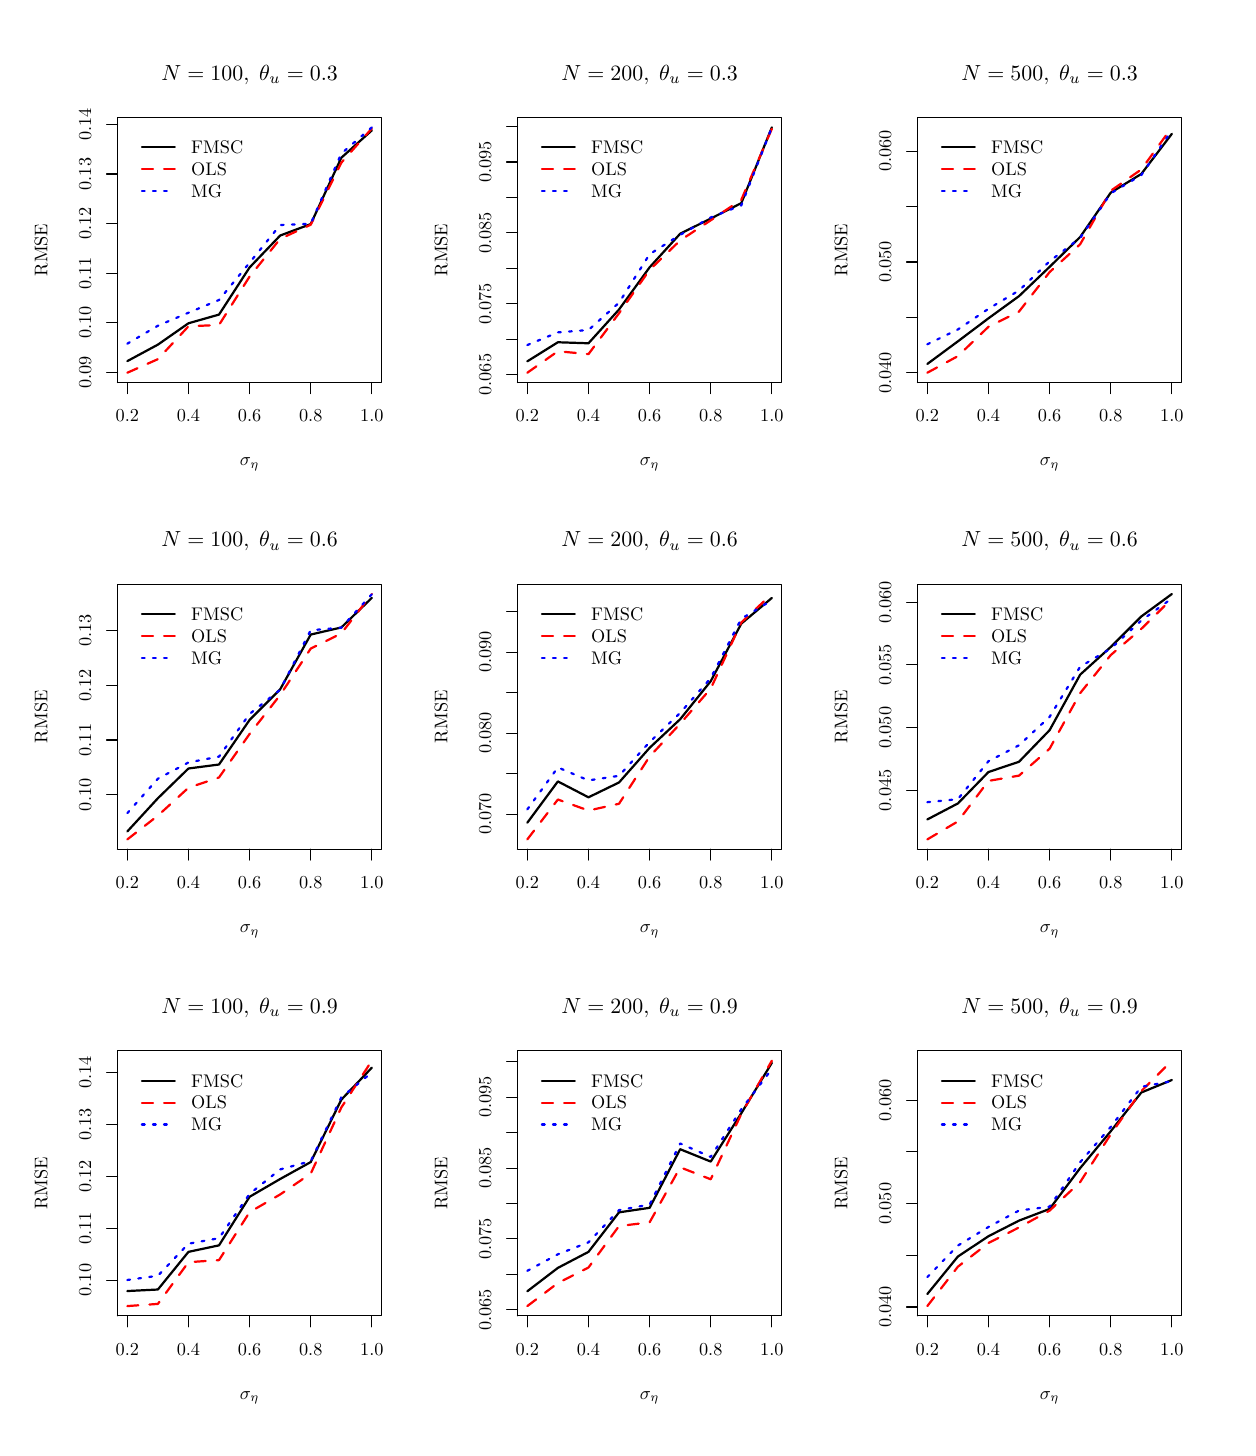
\begin{tikzpicture}[x=1pt,y=1pt]
\definecolor{fillColor}{RGB}{255,255,255}
\path[use as bounding box,fill=fillColor,fill opacity=0.00] (0,0) rectangle (433.62,505.89);
\begin{scope}
\path[clip] ( 32.47,377.65) rectangle (127.91,473.42);
\definecolor{drawColor}{RGB}{0,0,0}

\path[draw=drawColor,line width= 0.8pt,line join=round,line cap=round] ( 36.01,385.40) --
	( 47.05,391.35) --
	( 58.10,399.07) --
	( 69.14,402.21) --
	( 80.19,419.25) --
	( 91.24,430.77) --
	(102.28,434.91) --
	(113.33,458.88) --
	(124.37,468.77);
\end{scope}
\begin{scope}
\path[clip] (  0.00,  0.00) rectangle (433.62,505.89);
\definecolor{drawColor}{RGB}{0,0,0}

\path[draw=drawColor,line width= 0.4pt,line join=round,line cap=round] ( 36.01,377.65) -- (124.37,377.65);

\path[draw=drawColor,line width= 0.4pt,line join=round,line cap=round] ( 36.01,377.65) -- ( 36.01,373.69);

\path[draw=drawColor,line width= 0.4pt,line join=round,line cap=round] ( 58.10,377.65) -- ( 58.10,373.69);

\path[draw=drawColor,line width= 0.4pt,line join=round,line cap=round] ( 80.19,377.65) -- ( 80.19,373.69);

\path[draw=drawColor,line width= 0.4pt,line join=round,line cap=round] (102.28,377.65) -- (102.28,373.69);

\path[draw=drawColor,line width= 0.4pt,line join=round,line cap=round] (124.37,377.65) -- (124.37,373.69);

\node[text=drawColor,anchor=base,inner sep=0pt, outer sep=0pt, scale=  0.66] at ( 36.01,363.40) {0.2};

\node[text=drawColor,anchor=base,inner sep=0pt, outer sep=0pt, scale=  0.66] at ( 58.10,363.40) {0.4};

\node[text=drawColor,anchor=base,inner sep=0pt, outer sep=0pt, scale=  0.66] at ( 80.19,363.40) {0.6};

\node[text=drawColor,anchor=base,inner sep=0pt, outer sep=0pt, scale=  0.66] at (102.28,363.40) {0.8};

\node[text=drawColor,anchor=base,inner sep=0pt, outer sep=0pt, scale=  0.66] at (124.37,363.40) {1.0};

\path[draw=drawColor,line width= 0.4pt,line join=round,line cap=round] ( 32.47,381.36) -- ( 32.47,470.91);

\path[draw=drawColor,line width= 0.4pt,line join=round,line cap=round] ( 32.47,381.36) -- ( 28.51,381.36);

\path[draw=drawColor,line width= 0.4pt,line join=round,line cap=round] ( 32.47,399.27) -- ( 28.51,399.27);

\path[draw=drawColor,line width= 0.4pt,line join=round,line cap=round] ( 32.47,417.18) -- ( 28.51,417.18);

\path[draw=drawColor,line width= 0.4pt,line join=round,line cap=round] ( 32.47,435.09) -- ( 28.51,435.09);

\path[draw=drawColor,line width= 0.4pt,line join=round,line cap=round] ( 32.47,453.00) -- ( 28.51,453.00);

\path[draw=drawColor,line width= 0.4pt,line join=round,line cap=round] ( 32.47,470.91) -- ( 28.51,470.91);

\node[text=drawColor,rotate= 90.00,anchor=base,inner sep=0pt, outer sep=0pt, scale=  0.66] at ( 22.97,381.36) {0.09};

\node[text=drawColor,rotate= 90.00,anchor=base,inner sep=0pt, outer sep=0pt, scale=  0.66] at ( 22.97,399.27) {0.10};

\node[text=drawColor,rotate= 90.00,anchor=base,inner sep=0pt, outer sep=0pt, scale=  0.66] at ( 22.97,417.18) {0.11};

\node[text=drawColor,rotate= 90.00,anchor=base,inner sep=0pt, outer sep=0pt, scale=  0.66] at ( 22.97,435.09) {0.12};

\node[text=drawColor,rotate= 90.00,anchor=base,inner sep=0pt, outer sep=0pt, scale=  0.66] at ( 22.97,453.00) {0.13};

\node[text=drawColor,rotate= 90.00,anchor=base,inner sep=0pt, outer sep=0pt, scale=  0.66] at ( 22.97,470.91) {0.14};

\path[draw=drawColor,line width= 0.4pt,line join=round,line cap=round] ( 32.47,377.65) --
	(127.91,377.65) --
	(127.91,473.42) --
	( 32.47,473.42) --
	( 32.47,377.65);
\end{scope}
\begin{scope}
\path[clip] (  0.00,337.26) rectangle (144.54,505.89);
\definecolor{drawColor}{RGB}{0,0,0}

\node[text=drawColor,anchor=base,inner sep=0pt, outer sep=0pt, scale=  0.79] at ( 80.19,486.92) {\bfseries $N=100, \;\theta_u=0.3$};

\node[text=drawColor,anchor=base,inner sep=0pt, outer sep=0pt, scale=  0.66] at ( 80.19,347.56) {$\sigma_\eta$};

\node[text=drawColor,rotate= 90.00,anchor=base,inner sep=0pt, outer sep=0pt, scale=  0.66] at (  7.13,425.53) {RMSE};
\end{scope}
\begin{scope}
\path[clip] ( 32.47,377.65) rectangle (127.91,473.42);
\definecolor{drawColor}{RGB}{255,0,0}

\path[draw=drawColor,line width= 0.8pt,dash pattern=on 4pt off 4pt ,line join=round,line cap=round] ( 36.01,381.20) --
	( 47.05,386.10) --
	( 58.10,397.97) --
	( 69.14,398.46) --
	( 80.19,415.95) --
	( 91.24,429.58) --
	(102.28,434.68) --
	(113.33,457.09) --
	(124.37,469.48);
\definecolor{drawColor}{RGB}{0,0,255}

\path[draw=drawColor,line width= 0.8pt,dash pattern=on 1pt off 3pt ,line join=round,line cap=round] ( 36.01,391.70) --
	( 47.05,398.18) --
	( 58.10,402.88) --
	( 69.14,407.49) --
	( 80.19,420.96) --
	( 91.24,434.58) --
	(102.28,435.02) --
	(113.33,460.39) --
	(124.37,469.87);
\definecolor{drawColor}{RGB}{0,0,0}

\path[draw=drawColor,line width= 0.8pt,line join=round,line cap=round] ( 41.28,462.63) -- ( 53.16,462.63);
\definecolor{drawColor}{RGB}{255,0,0}

\path[draw=drawColor,line width= 0.8pt,dash pattern=on 4pt off 4pt ,line join=round,line cap=round] ( 41.28,454.71) -- ( 53.16,454.71);
\definecolor{drawColor}{RGB}{0,0,255}

\path[draw=drawColor,line width= 0.8pt,dash pattern=on 1pt off 3pt ,line join=round,line cap=round] ( 41.28,446.79) -- ( 53.16,446.79);
\definecolor{drawColor}{RGB}{0,0,0}

\node[text=drawColor,anchor=base west,inner sep=0pt, outer sep=0pt, scale=  0.66] at ( 59.10,460.35) {FMSC};

\node[text=drawColor,anchor=base west,inner sep=0pt, outer sep=0pt, scale=  0.66] at ( 59.10,452.43) {OLS};

\node[text=drawColor,anchor=base west,inner sep=0pt, outer sep=0pt, scale=  0.66] at ( 59.10,444.51) {MG};
\end{scope}
\begin{scope}
\path[clip] (177.01,377.65) rectangle (272.45,473.42);
\definecolor{drawColor}{RGB}{0,0,0}

\path[draw=drawColor,line width= 0.8pt,line join=round,line cap=round] (180.55,385.32) --
	(191.59,392.21) --
	(202.64,391.84) --
	(213.68,404.04) --
	(224.73,419.28) --
	(235.78,431.43) --
	(246.82,436.91) --
	(257.87,442.50) --
	(268.91,469.87);
\end{scope}
\begin{scope}
\path[clip] (  0.00,  0.00) rectangle (433.62,505.89);
\definecolor{drawColor}{RGB}{0,0,0}

\path[draw=drawColor,line width= 0.4pt,line join=round,line cap=round] (180.55,377.65) -- (268.91,377.65);

\path[draw=drawColor,line width= 0.4pt,line join=round,line cap=round] (180.55,377.65) -- (180.55,373.69);

\path[draw=drawColor,line width= 0.4pt,line join=round,line cap=round] (202.64,377.65) -- (202.64,373.69);

\path[draw=drawColor,line width= 0.4pt,line join=round,line cap=round] (224.73,377.65) -- (224.73,373.69);

\path[draw=drawColor,line width= 0.4pt,line join=round,line cap=round] (246.82,377.65) -- (246.82,373.69);

\path[draw=drawColor,line width= 0.4pt,line join=round,line cap=round] (268.91,377.65) -- (268.91,373.69);

\node[text=drawColor,anchor=base,inner sep=0pt, outer sep=0pt, scale=  0.66] at (180.55,363.40) {0.2};

\node[text=drawColor,anchor=base,inner sep=0pt, outer sep=0pt, scale=  0.66] at (202.64,363.40) {0.4};

\node[text=drawColor,anchor=base,inner sep=0pt, outer sep=0pt, scale=  0.66] at (224.73,363.40) {0.6};

\node[text=drawColor,anchor=base,inner sep=0pt, outer sep=0pt, scale=  0.66] at (246.82,363.40) {0.8};

\node[text=drawColor,anchor=base,inner sep=0pt, outer sep=0pt, scale=  0.66] at (268.91,363.40) {1.0};

\path[draw=drawColor,line width= 0.4pt,line join=round,line cap=round] (177.01,380.55) -- (177.01,470.14);

\path[draw=drawColor,line width= 0.4pt,line join=round,line cap=round] (177.01,380.55) -- (173.05,380.55);

\path[draw=drawColor,line width= 0.4pt,line join=round,line cap=round] (177.01,393.35) -- (173.05,393.35);

\path[draw=drawColor,line width= 0.4pt,line join=round,line cap=round] (177.01,406.15) -- (173.05,406.15);

\path[draw=drawColor,line width= 0.4pt,line join=round,line cap=round] (177.01,418.95) -- (173.05,418.95);

\path[draw=drawColor,line width= 0.4pt,line join=round,line cap=round] (177.01,431.75) -- (173.05,431.75);

\path[draw=drawColor,line width= 0.4pt,line join=round,line cap=round] (177.01,444.54) -- (173.05,444.54);

\path[draw=drawColor,line width= 0.4pt,line join=round,line cap=round] (177.01,457.34) -- (173.05,457.34);

\path[draw=drawColor,line width= 0.4pt,line join=round,line cap=round] (177.01,470.14) -- (173.05,470.14);

\node[text=drawColor,rotate= 90.00,anchor=base,inner sep=0pt, outer sep=0pt, scale=  0.66] at (167.51,380.55) {0.065};

\node[text=drawColor,rotate= 90.00,anchor=base,inner sep=0pt, outer sep=0pt, scale=  0.66] at (167.51,406.15) {0.075};

\node[text=drawColor,rotate= 90.00,anchor=base,inner sep=0pt, outer sep=0pt, scale=  0.66] at (167.51,431.75) {0.085};

\node[text=drawColor,rotate= 90.00,anchor=base,inner sep=0pt, outer sep=0pt, scale=  0.66] at (167.51,457.34) {0.095};

\path[draw=drawColor,line width= 0.4pt,line join=round,line cap=round] (177.01,377.65) --
	(272.45,377.65) --
	(272.45,473.42) --
	(177.01,473.42) --
	(177.01,377.65);
\end{scope}
\begin{scope}
\path[clip] (144.54,337.26) rectangle (289.08,505.89);
\definecolor{drawColor}{RGB}{0,0,0}

\node[text=drawColor,anchor=base,inner sep=0pt, outer sep=0pt, scale=  0.79] at (224.73,486.92) {\bfseries $N=200, \;\theta_u=0.3$};

\node[text=drawColor,anchor=base,inner sep=0pt, outer sep=0pt, scale=  0.66] at (224.73,347.56) {$\sigma_\eta$};

\node[text=drawColor,rotate= 90.00,anchor=base,inner sep=0pt, outer sep=0pt, scale=  0.66] at (151.67,425.53) {RMSE};
\end{scope}
\begin{scope}
\path[clip] (177.01,377.65) rectangle (272.45,473.42);
\definecolor{drawColor}{RGB}{255,0,0}

\path[draw=drawColor,line width= 0.8pt,dash pattern=on 4pt off 4pt ,line join=round,line cap=round] (180.55,381.20) --
	(191.59,388.96) --
	(202.64,387.92) --
	(213.68,402.68) --
	(224.73,418.35) --
	(235.78,429.02) --
	(246.82,436.27) --
	(257.87,443.71) --
	(268.91,469.35);
\definecolor{drawColor}{RGB}{0,0,255}

\path[draw=drawColor,line width= 0.8pt,dash pattern=on 1pt off 3pt ,line join=round,line cap=round] (180.55,391.20) --
	(191.59,395.78) --
	(202.64,396.63) --
	(213.68,406.49) --
	(224.73,424.02) --
	(235.78,431.02) --
	(246.82,437.30) --
	(257.87,441.69) --
	(268.91,469.83);
\definecolor{drawColor}{RGB}{0,0,0}

\path[draw=drawColor,line width= 0.8pt,line join=round,line cap=round] (185.82,462.63) -- (197.70,462.63);
\definecolor{drawColor}{RGB}{255,0,0}

\path[draw=drawColor,line width= 0.8pt,dash pattern=on 4pt off 4pt ,line join=round,line cap=round] (185.82,454.71) -- (197.70,454.71);
\definecolor{drawColor}{RGB}{0,0,255}

\path[draw=drawColor,line width= 0.8pt,dash pattern=on 1pt off 3pt ,line join=round,line cap=round] (185.82,446.79) -- (197.70,446.79);
\definecolor{drawColor}{RGB}{0,0,0}

\node[text=drawColor,anchor=base west,inner sep=0pt, outer sep=0pt, scale=  0.66] at (203.64,460.35) {FMSC};

\node[text=drawColor,anchor=base west,inner sep=0pt, outer sep=0pt, scale=  0.66] at (203.64,452.43) {OLS};

\node[text=drawColor,anchor=base west,inner sep=0pt, outer sep=0pt, scale=  0.66] at (203.64,444.51) {MG};
\end{scope}
\begin{scope}
\path[clip] (321.55,377.65) rectangle (416.99,473.42);
\definecolor{drawColor}{RGB}{0,0,0}

\path[draw=drawColor,line width= 0.8pt,line join=round,line cap=round] (325.09,384.37) --
	(336.13,392.54) --
	(347.18,400.86) --
	(358.22,408.88) --
	(369.27,419.45) --
	(380.32,430.26) --
	(391.36,446.26) --
	(402.41,453.03) --
	(413.45,467.53);
\end{scope}
\begin{scope}
\path[clip] (  0.00,  0.00) rectangle (433.62,505.89);
\definecolor{drawColor}{RGB}{0,0,0}

\path[draw=drawColor,line width= 0.4pt,line join=round,line cap=round] (325.09,377.65) -- (413.45,377.65);

\path[draw=drawColor,line width= 0.4pt,line join=round,line cap=round] (325.09,377.65) -- (325.09,373.69);

\path[draw=drawColor,line width= 0.4pt,line join=round,line cap=round] (347.18,377.65) -- (347.18,373.69);

\path[draw=drawColor,line width= 0.4pt,line join=round,line cap=round] (369.27,377.65) -- (369.27,373.69);

\path[draw=drawColor,line width= 0.4pt,line join=round,line cap=round] (391.36,377.65) -- (391.36,373.69);

\path[draw=drawColor,line width= 0.4pt,line join=round,line cap=round] (413.45,377.65) -- (413.45,373.69);

\node[text=drawColor,anchor=base,inner sep=0pt, outer sep=0pt, scale=  0.66] at (325.09,363.40) {0.2};

\node[text=drawColor,anchor=base,inner sep=0pt, outer sep=0pt, scale=  0.66] at (347.18,363.40) {0.4};

\node[text=drawColor,anchor=base,inner sep=0pt, outer sep=0pt, scale=  0.66] at (369.27,363.40) {0.6};

\node[text=drawColor,anchor=base,inner sep=0pt, outer sep=0pt, scale=  0.66] at (391.36,363.40) {0.8};

\node[text=drawColor,anchor=base,inner sep=0pt, outer sep=0pt, scale=  0.66] at (413.45,363.40) {1.0};

\path[draw=drawColor,line width= 0.4pt,line join=round,line cap=round] (321.55,381.13) -- (321.55,461.30);

\path[draw=drawColor,line width= 0.4pt,line join=round,line cap=round] (321.55,381.13) -- (317.59,381.13);

\path[draw=drawColor,line width= 0.4pt,line join=round,line cap=round] (321.55,401.17) -- (317.59,401.17);

\path[draw=drawColor,line width= 0.4pt,line join=round,line cap=round] (321.55,421.22) -- (317.59,421.22);

\path[draw=drawColor,line width= 0.4pt,line join=round,line cap=round] (321.55,441.26) -- (317.59,441.26);

\path[draw=drawColor,line width= 0.4pt,line join=round,line cap=round] (321.55,461.30) -- (317.59,461.30);

\node[text=drawColor,rotate= 90.00,anchor=base,inner sep=0pt, outer sep=0pt, scale=  0.66] at (312.05,381.13) {0.040};

\node[text=drawColor,rotate= 90.00,anchor=base,inner sep=0pt, outer sep=0pt, scale=  0.66] at (312.05,421.22) {0.050};

\node[text=drawColor,rotate= 90.00,anchor=base,inner sep=0pt, outer sep=0pt, scale=  0.66] at (312.05,461.30) {0.060};

\path[draw=drawColor,line width= 0.4pt,line join=round,line cap=round] (321.55,377.65) --
	(416.99,377.65) --
	(416.99,473.42) --
	(321.55,473.42) --
	(321.55,377.65);
\end{scope}
\begin{scope}
\path[clip] (289.08,337.26) rectangle (433.62,505.89);
\definecolor{drawColor}{RGB}{0,0,0}

\node[text=drawColor,anchor=base,inner sep=0pt, outer sep=0pt, scale=  0.79] at (369.27,486.92) {\bfseries $N=500, \;\theta_u=0.3$};

\node[text=drawColor,anchor=base,inner sep=0pt, outer sep=0pt, scale=  0.66] at (369.27,347.56) {$\sigma_\eta$};

\node[text=drawColor,rotate= 90.00,anchor=base,inner sep=0pt, outer sep=0pt, scale=  0.66] at (296.21,425.53) {RMSE};
\end{scope}
\begin{scope}
\path[clip] (321.55,377.65) rectangle (416.99,473.42);
\definecolor{drawColor}{RGB}{255,0,0}

\path[draw=drawColor,line width= 0.8pt,dash pattern=on 4pt off 4pt ,line join=round,line cap=round] (325.09,381.20) --
	(336.13,387.20) --
	(347.18,397.80) --
	(358.22,403.29) --
	(369.27,417.56) --
	(380.32,427.63) --
	(391.36,446.94) --
	(402.41,454.65) --
	(413.45,469.87);
\definecolor{drawColor}{RGB}{0,0,255}

\path[draw=drawColor,line width= 0.8pt,dash pattern=on 1pt off 3pt ,line join=round,line cap=round] (325.09,391.47) --
	(336.13,396.84) --
	(347.18,404.30) --
	(358.22,410.92) --
	(369.27,421.46) --
	(380.32,429.92) --
	(391.36,446.02) --
	(402.41,452.62) --
	(413.45,468.82);
\definecolor{drawColor}{RGB}{0,0,0}

\path[draw=drawColor,line width= 0.8pt,line join=round,line cap=round] (330.36,462.63) -- (342.24,462.63);
\definecolor{drawColor}{RGB}{255,0,0}

\path[draw=drawColor,line width= 0.8pt,dash pattern=on 4pt off 4pt ,line join=round,line cap=round] (330.36,454.71) -- (342.24,454.71);
\definecolor{drawColor}{RGB}{0,0,255}

\path[draw=drawColor,line width= 0.8pt,dash pattern=on 1pt off 3pt ,line join=round,line cap=round] (330.36,446.79) -- (342.24,446.79);
\definecolor{drawColor}{RGB}{0,0,0}

\node[text=drawColor,anchor=base west,inner sep=0pt, outer sep=0pt, scale=  0.66] at (348.18,460.35) {FMSC};

\node[text=drawColor,anchor=base west,inner sep=0pt, outer sep=0pt, scale=  0.66] at (348.18,452.43) {OLS};

\node[text=drawColor,anchor=base west,inner sep=0pt, outer sep=0pt, scale=  0.66] at (348.18,444.51) {MG};
\end{scope}
\begin{scope}
\path[clip] ( 32.47,209.02) rectangle (127.91,304.79);
\definecolor{drawColor}{RGB}{0,0,0}

\path[draw=drawColor,line width= 0.8pt,line join=round,line cap=round] ( 36.01,215.44) --
	( 47.05,227.44) --
	( 58.10,238.19) --
	( 69.14,239.63) --
	( 80.19,255.74) --
	( 91.24,266.81) --
	(102.28,286.59) --
	(113.33,289.15) --
	(124.37,299.86);
\end{scope}
\begin{scope}
\path[clip] (  0.00,  0.00) rectangle (433.62,505.89);
\definecolor{drawColor}{RGB}{0,0,0}

\path[draw=drawColor,line width= 0.4pt,line join=round,line cap=round] ( 36.01,209.02) -- (124.37,209.02);

\path[draw=drawColor,line width= 0.4pt,line join=round,line cap=round] ( 36.01,209.02) -- ( 36.01,205.06);

\path[draw=drawColor,line width= 0.4pt,line join=round,line cap=round] ( 58.10,209.02) -- ( 58.10,205.06);

\path[draw=drawColor,line width= 0.4pt,line join=round,line cap=round] ( 80.19,209.02) -- ( 80.19,205.06);

\path[draw=drawColor,line width= 0.4pt,line join=round,line cap=round] (102.28,209.02) -- (102.28,205.06);

\path[draw=drawColor,line width= 0.4pt,line join=round,line cap=round] (124.37,209.02) -- (124.37,205.06);

\node[text=drawColor,anchor=base,inner sep=0pt, outer sep=0pt, scale=  0.66] at ( 36.01,194.77) {0.2};

\node[text=drawColor,anchor=base,inner sep=0pt, outer sep=0pt, scale=  0.66] at ( 58.10,194.77) {0.4};

\node[text=drawColor,anchor=base,inner sep=0pt, outer sep=0pt, scale=  0.66] at ( 80.19,194.77) {0.6};

\node[text=drawColor,anchor=base,inner sep=0pt, outer sep=0pt, scale=  0.66] at (102.28,194.77) {0.8};

\node[text=drawColor,anchor=base,inner sep=0pt, outer sep=0pt, scale=  0.66] at (124.37,194.77) {1.0};

\path[draw=drawColor,line width= 0.4pt,line join=round,line cap=round] ( 32.47,228.70) -- ( 32.47,288.06);

\path[draw=drawColor,line width= 0.4pt,line join=round,line cap=round] ( 32.47,228.70) -- ( 28.51,228.70);

\path[draw=drawColor,line width= 0.4pt,line join=round,line cap=round] ( 32.47,248.49) -- ( 28.51,248.49);

\path[draw=drawColor,line width= 0.4pt,line join=round,line cap=round] ( 32.47,268.27) -- ( 28.51,268.27);

\path[draw=drawColor,line width= 0.4pt,line join=round,line cap=round] ( 32.47,288.06) -- ( 28.51,288.06);

\node[text=drawColor,rotate= 90.00,anchor=base,inner sep=0pt, outer sep=0pt, scale=  0.66] at ( 22.97,228.70) {0.10};

\node[text=drawColor,rotate= 90.00,anchor=base,inner sep=0pt, outer sep=0pt, scale=  0.66] at ( 22.97,248.49) {0.11};

\node[text=drawColor,rotate= 90.00,anchor=base,inner sep=0pt, outer sep=0pt, scale=  0.66] at ( 22.97,268.27) {0.12};

\node[text=drawColor,rotate= 90.00,anchor=base,inner sep=0pt, outer sep=0pt, scale=  0.66] at ( 22.97,288.06) {0.13};

\path[draw=drawColor,line width= 0.4pt,line join=round,line cap=round] ( 32.47,209.02) --
	(127.91,209.02) --
	(127.91,304.79) --
	( 32.47,304.79) --
	( 32.47,209.02);
\end{scope}
\begin{scope}
\path[clip] (  0.00,168.63) rectangle (144.54,337.26);
\definecolor{drawColor}{RGB}{0,0,0}

\node[text=drawColor,anchor=base,inner sep=0pt, outer sep=0pt, scale=  0.79] at ( 80.19,318.29) {\bfseries $N=100, \;\theta_u=0.6$};

\node[text=drawColor,anchor=base,inner sep=0pt, outer sep=0pt, scale=  0.66] at ( 80.19,178.93) {$\sigma_\eta$};

\node[text=drawColor,rotate= 90.00,anchor=base,inner sep=0pt, outer sep=0pt, scale=  0.66] at (  7.13,256.90) {RMSE};
\end{scope}
\begin{scope}
\path[clip] ( 32.47,209.02) rectangle (127.91,304.79);
\definecolor{drawColor}{RGB}{255,0,0}

\path[draw=drawColor,line width= 0.8pt,dash pattern=on 4pt off 4pt ,line join=round,line cap=round] ( 36.01,212.57) --
	( 47.05,221.15) --
	( 58.10,231.24) --
	( 69.14,234.95) --
	( 80.19,250.67) --
	( 91.24,264.74) --
	(102.28,281.51) --
	(113.33,287.01) --
	(124.37,301.24);
\definecolor{drawColor}{RGB}{0,0,255}

\path[draw=drawColor,line width= 0.8pt,dash pattern=on 1pt off 3pt ,line join=round,line cap=round] ( 36.01,222.06) --
	( 47.05,234.50) --
	( 58.10,240.37) --
	( 69.14,242.49) --
	( 80.19,257.90) --
	( 91.24,266.66) --
	(102.28,288.14) --
	(113.33,289.08) --
	(124.37,301.17);
\definecolor{drawColor}{RGB}{0,0,0}

\path[draw=drawColor,line width= 0.8pt,line join=round,line cap=round] ( 41.28,294.00) -- ( 53.16,294.00);
\definecolor{drawColor}{RGB}{255,0,0}

\path[draw=drawColor,line width= 0.8pt,dash pattern=on 4pt off 4pt ,line join=round,line cap=round] ( 41.28,286.08) -- ( 53.16,286.08);
\definecolor{drawColor}{RGB}{0,0,255}

\path[draw=drawColor,line width= 0.8pt,dash pattern=on 1pt off 3pt ,line join=round,line cap=round] ( 41.28,278.16) -- ( 53.16,278.16);
\definecolor{drawColor}{RGB}{0,0,0}

\node[text=drawColor,anchor=base west,inner sep=0pt, outer sep=0pt, scale=  0.66] at ( 59.10,291.72) {FMSC};

\node[text=drawColor,anchor=base west,inner sep=0pt, outer sep=0pt, scale=  0.66] at ( 59.10,283.80) {OLS};

\node[text=drawColor,anchor=base west,inner sep=0pt, outer sep=0pt, scale=  0.66] at ( 59.10,275.88) {MG};
\end{scope}
\begin{scope}
\path[clip] (177.01,209.02) rectangle (272.45,304.79);
\definecolor{drawColor}{RGB}{0,0,0}

\path[draw=drawColor,line width= 0.8pt,line join=round,line cap=round] (180.55,218.60) --
	(191.59,233.52) --
	(202.64,227.78) --
	(213.68,233.14) --
	(224.73,245.65) --
	(235.78,256.00) --
	(246.82,269.74) --
	(257.87,290.54) --
	(268.91,299.82);
\end{scope}
\begin{scope}
\path[clip] (  0.00,  0.00) rectangle (433.62,505.89);
\definecolor{drawColor}{RGB}{0,0,0}

\path[draw=drawColor,line width= 0.4pt,line join=round,line cap=round] (180.55,209.02) -- (268.91,209.02);

\path[draw=drawColor,line width= 0.4pt,line join=round,line cap=round] (180.55,209.02) -- (180.55,205.06);

\path[draw=drawColor,line width= 0.4pt,line join=round,line cap=round] (202.64,209.02) -- (202.64,205.06);

\path[draw=drawColor,line width= 0.4pt,line join=round,line cap=round] (224.73,209.02) -- (224.73,205.06);

\path[draw=drawColor,line width= 0.4pt,line join=round,line cap=round] (246.82,209.02) -- (246.82,205.06);

\path[draw=drawColor,line width= 0.4pt,line join=round,line cap=round] (268.91,209.02) -- (268.91,205.06);

\node[text=drawColor,anchor=base,inner sep=0pt, outer sep=0pt, scale=  0.66] at (180.55,194.77) {0.2};

\node[text=drawColor,anchor=base,inner sep=0pt, outer sep=0pt, scale=  0.66] at (202.64,194.77) {0.4};

\node[text=drawColor,anchor=base,inner sep=0pt, outer sep=0pt, scale=  0.66] at (224.73,194.77) {0.6};

\node[text=drawColor,anchor=base,inner sep=0pt, outer sep=0pt, scale=  0.66] at (246.82,194.77) {0.8};

\node[text=drawColor,anchor=base,inner sep=0pt, outer sep=0pt, scale=  0.66] at (268.91,194.77) {1.0};

\path[draw=drawColor,line width= 0.4pt,line join=round,line cap=round] (177.01,221.68) -- (177.01,294.85);

\path[draw=drawColor,line width= 0.4pt,line join=round,line cap=round] (177.01,221.68) -- (173.05,221.68);

\path[draw=drawColor,line width= 0.4pt,line join=round,line cap=round] (177.01,236.31) -- (173.05,236.31);

\path[draw=drawColor,line width= 0.4pt,line join=round,line cap=round] (177.01,250.95) -- (173.05,250.95);

\path[draw=drawColor,line width= 0.4pt,line join=round,line cap=round] (177.01,265.58) -- (173.05,265.58);

\path[draw=drawColor,line width= 0.4pt,line join=round,line cap=round] (177.01,280.22) -- (173.05,280.22);

\path[draw=drawColor,line width= 0.4pt,line join=round,line cap=round] (177.01,294.85) -- (173.05,294.85);

\node[text=drawColor,rotate= 90.00,anchor=base,inner sep=0pt, outer sep=0pt, scale=  0.66] at (167.51,221.68) {0.070};

\node[text=drawColor,rotate= 90.00,anchor=base,inner sep=0pt, outer sep=0pt, scale=  0.66] at (167.51,250.95) {0.080};

\node[text=drawColor,rotate= 90.00,anchor=base,inner sep=0pt, outer sep=0pt, scale=  0.66] at (167.51,280.22) {0.090};

\path[draw=drawColor,line width= 0.4pt,line join=round,line cap=round] (177.01,209.02) --
	(272.45,209.02) --
	(272.45,304.79) --
	(177.01,304.79) --
	(177.01,209.02);
\end{scope}
\begin{scope}
\path[clip] (144.54,168.63) rectangle (289.08,337.26);
\definecolor{drawColor}{RGB}{0,0,0}

\node[text=drawColor,anchor=base,inner sep=0pt, outer sep=0pt, scale=  0.79] at (224.73,318.29) {\bfseries $N=200, \;\theta_u=0.6$};

\node[text=drawColor,anchor=base,inner sep=0pt, outer sep=0pt, scale=  0.66] at (224.73,178.93) {$\sigma_\eta$};

\node[text=drawColor,rotate= 90.00,anchor=base,inner sep=0pt, outer sep=0pt, scale=  0.66] at (151.67,256.90) {RMSE};
\end{scope}
\begin{scope}
\path[clip] (177.01,209.02) rectangle (272.45,304.79);
\definecolor{drawColor}{RGB}{255,0,0}

\path[draw=drawColor,line width= 0.8pt,dash pattern=on 4pt off 4pt ,line join=round,line cap=round] (180.55,212.57) --
	(191.59,226.98) --
	(202.64,223.00) --
	(213.68,225.45) --
	(224.73,242.51) --
	(235.78,254.36) --
	(246.82,267.06) --
	(257.87,290.96) --
	(268.91,301.24);
\definecolor{drawColor}{RGB}{0,0,255}

\path[draw=drawColor,line width= 0.8pt,dash pattern=on 1pt off 3pt ,line join=round,line cap=round] (180.55,223.42) --
	(191.59,238.58) --
	(202.64,233.89) --
	(213.68,235.54) --
	(224.73,247.74) --
	(235.78,258.28) --
	(246.82,270.86) --
	(257.87,292.30) --
	(268.91,299.00);
\definecolor{drawColor}{RGB}{0,0,0}

\path[draw=drawColor,line width= 0.8pt,line join=round,line cap=round] (185.82,294.00) -- (197.70,294.00);
\definecolor{drawColor}{RGB}{255,0,0}

\path[draw=drawColor,line width= 0.8pt,dash pattern=on 4pt off 4pt ,line join=round,line cap=round] (185.82,286.08) -- (197.70,286.08);
\definecolor{drawColor}{RGB}{0,0,255}

\path[draw=drawColor,line width= 0.8pt,dash pattern=on 1pt off 3pt ,line join=round,line cap=round] (185.82,278.16) -- (197.70,278.16);
\definecolor{drawColor}{RGB}{0,0,0}

\node[text=drawColor,anchor=base west,inner sep=0pt, outer sep=0pt, scale=  0.66] at (203.64,291.72) {FMSC};

\node[text=drawColor,anchor=base west,inner sep=0pt, outer sep=0pt, scale=  0.66] at (203.64,283.80) {OLS};

\node[text=drawColor,anchor=base west,inner sep=0pt, outer sep=0pt, scale=  0.66] at (203.64,275.88) {MG};
\end{scope}
\begin{scope}
\path[clip] (321.55,209.02) rectangle (416.99,304.79);
\definecolor{drawColor}{RGB}{0,0,0}

\path[draw=drawColor,line width= 0.8pt,line join=round,line cap=round] (325.09,219.78) --
	(336.13,225.56) --
	(347.18,236.91) --
	(358.22,240.63) --
	(369.27,252.04) --
	(380.32,272.11) --
	(391.36,282.11) --
	(402.41,293.13) --
	(413.45,301.24);
\end{scope}
\begin{scope}
\path[clip] (  0.00,  0.00) rectangle (433.62,505.89);
\definecolor{drawColor}{RGB}{0,0,0}

\path[draw=drawColor,line width= 0.4pt,line join=round,line cap=round] (325.09,209.02) -- (413.45,209.02);

\path[draw=drawColor,line width= 0.4pt,line join=round,line cap=round] (325.09,209.02) -- (325.09,205.06);

\path[draw=drawColor,line width= 0.4pt,line join=round,line cap=round] (347.18,209.02) -- (347.18,205.06);

\path[draw=drawColor,line width= 0.4pt,line join=round,line cap=round] (369.27,209.02) -- (369.27,205.06);

\path[draw=drawColor,line width= 0.4pt,line join=round,line cap=round] (391.36,209.02) -- (391.36,205.06);

\path[draw=drawColor,line width= 0.4pt,line join=round,line cap=round] (413.45,209.02) -- (413.45,205.06);

\node[text=drawColor,anchor=base,inner sep=0pt, outer sep=0pt, scale=  0.66] at (325.09,194.77) {0.2};

\node[text=drawColor,anchor=base,inner sep=0pt, outer sep=0pt, scale=  0.66] at (347.18,194.77) {0.4};

\node[text=drawColor,anchor=base,inner sep=0pt, outer sep=0pt, scale=  0.66] at (369.27,194.77) {0.6};

\node[text=drawColor,anchor=base,inner sep=0pt, outer sep=0pt, scale=  0.66] at (391.36,194.77) {0.8};

\node[text=drawColor,anchor=base,inner sep=0pt, outer sep=0pt, scale=  0.66] at (413.45,194.77) {1.0};

\path[draw=drawColor,line width= 0.4pt,line join=round,line cap=round] (321.55,230.30) -- (321.55,298.27);

\path[draw=drawColor,line width= 0.4pt,line join=round,line cap=round] (321.55,230.30) -- (317.59,230.30);

\path[draw=drawColor,line width= 0.4pt,line join=round,line cap=round] (321.55,252.96) -- (317.59,252.96);

\path[draw=drawColor,line width= 0.4pt,line join=round,line cap=round] (321.55,275.61) -- (317.59,275.61);

\path[draw=drawColor,line width= 0.4pt,line join=round,line cap=round] (321.55,298.27) -- (317.59,298.27);

\node[text=drawColor,rotate= 90.00,anchor=base,inner sep=0pt, outer sep=0pt, scale=  0.66] at (312.05,230.30) {0.045};

\node[text=drawColor,rotate= 90.00,anchor=base,inner sep=0pt, outer sep=0pt, scale=  0.66] at (312.05,252.96) {0.050};

\node[text=drawColor,rotate= 90.00,anchor=base,inner sep=0pt, outer sep=0pt, scale=  0.66] at (312.05,275.61) {0.055};

\node[text=drawColor,rotate= 90.00,anchor=base,inner sep=0pt, outer sep=0pt, scale=  0.66] at (312.05,298.27) {0.060};

\path[draw=drawColor,line width= 0.4pt,line join=round,line cap=round] (321.55,209.02) --
	(416.99,209.02) --
	(416.99,304.79) --
	(321.55,304.79) --
	(321.55,209.02);
\end{scope}
\begin{scope}
\path[clip] (289.08,168.63) rectangle (433.62,337.26);
\definecolor{drawColor}{RGB}{0,0,0}

\node[text=drawColor,anchor=base,inner sep=0pt, outer sep=0pt, scale=  0.79] at (369.27,318.29) {\bfseries $N=500, \;\theta_u=0.6$};

\node[text=drawColor,anchor=base,inner sep=0pt, outer sep=0pt, scale=  0.66] at (369.27,178.93) {$\sigma_\eta$};

\node[text=drawColor,rotate= 90.00,anchor=base,inner sep=0pt, outer sep=0pt, scale=  0.66] at (296.21,256.90) {RMSE};
\end{scope}
\begin{scope}
\path[clip] (321.55,209.02) rectangle (416.99,304.79);
\definecolor{drawColor}{RGB}{255,0,0}

\path[draw=drawColor,line width= 0.8pt,dash pattern=on 4pt off 4pt ,line join=round,line cap=round] (325.09,212.57) --
	(336.13,219.07) --
	(347.18,233.71) --
	(358.22,235.61) --
	(369.27,245.34) --
	(380.32,265.42) --
	(391.36,279.18) --
	(402.41,288.65) --
	(413.45,299.50);
\definecolor{drawColor}{RGB}{0,0,255}

\path[draw=drawColor,line width= 0.8pt,dash pattern=on 1pt off 3pt ,line join=round,line cap=round] (325.09,226.02) --
	(336.13,227.10) --
	(347.18,240.81) --
	(358.22,246.58) --
	(369.27,256.85) --
	(380.32,274.98) --
	(391.36,281.52) --
	(402.41,291.67) --
	(413.45,299.66);
\definecolor{drawColor}{RGB}{0,0,0}

\path[draw=drawColor,line width= 0.8pt,line join=round,line cap=round] (330.36,294.00) -- (342.24,294.00);
\definecolor{drawColor}{RGB}{255,0,0}

\path[draw=drawColor,line width= 0.8pt,dash pattern=on 4pt off 4pt ,line join=round,line cap=round] (330.36,286.08) -- (342.24,286.08);
\definecolor{drawColor}{RGB}{0,0,255}

\path[draw=drawColor,line width= 0.8pt,dash pattern=on 1pt off 3pt ,line join=round,line cap=round] (330.36,278.16) -- (342.24,278.16);
\definecolor{drawColor}{RGB}{0,0,0}

\node[text=drawColor,anchor=base west,inner sep=0pt, outer sep=0pt, scale=  0.66] at (348.18,291.72) {FMSC};

\node[text=drawColor,anchor=base west,inner sep=0pt, outer sep=0pt, scale=  0.66] at (348.18,283.80) {OLS};

\node[text=drawColor,anchor=base west,inner sep=0pt, outer sep=0pt, scale=  0.66] at (348.18,275.88) {MG};
\end{scope}
\begin{scope}
\path[clip] ( 32.47, 40.39) rectangle (127.91,136.16);
\definecolor{drawColor}{RGB}{0,0,0}

\path[draw=drawColor,line width= 0.8pt,line join=round,line cap=round] ( 36.01, 49.37) --
	( 47.05, 49.92) --
	( 58.10, 63.53) --
	( 69.14, 65.88) --
	( 80.19, 83.43) --
	( 91.24, 89.86) --
	(102.28, 95.97) --
	(113.33,118.51) --
	(124.37,130.10);
\end{scope}
\begin{scope}
\path[clip] (  0.00,  0.00) rectangle (433.62,505.89);
\definecolor{drawColor}{RGB}{0,0,0}

\path[draw=drawColor,line width= 0.4pt,line join=round,line cap=round] ( 36.01, 40.39) -- (124.37, 40.39);

\path[draw=drawColor,line width= 0.4pt,line join=round,line cap=round] ( 36.01, 40.39) -- ( 36.01, 36.43);

\path[draw=drawColor,line width= 0.4pt,line join=round,line cap=round] ( 58.10, 40.39) -- ( 58.10, 36.43);

\path[draw=drawColor,line width= 0.4pt,line join=round,line cap=round] ( 80.19, 40.39) -- ( 80.19, 36.43);

\path[draw=drawColor,line width= 0.4pt,line join=round,line cap=round] (102.28, 40.39) -- (102.28, 36.43);

\path[draw=drawColor,line width= 0.4pt,line join=round,line cap=round] (124.37, 40.39) -- (124.37, 36.43);

\node[text=drawColor,anchor=base,inner sep=0pt, outer sep=0pt, scale=  0.66] at ( 36.01, 26.14) {0.2};

\node[text=drawColor,anchor=base,inner sep=0pt, outer sep=0pt, scale=  0.66] at ( 58.10, 26.14) {0.4};

\node[text=drawColor,anchor=base,inner sep=0pt, outer sep=0pt, scale=  0.66] at ( 80.19, 26.14) {0.6};

\node[text=drawColor,anchor=base,inner sep=0pt, outer sep=0pt, scale=  0.66] at (102.28, 26.14) {0.8};

\node[text=drawColor,anchor=base,inner sep=0pt, outer sep=0pt, scale=  0.66] at (124.37, 26.14) {1.0};

\path[draw=drawColor,line width= 0.4pt,line join=round,line cap=round] ( 32.47, 53.33) -- ( 32.47,128.32);

\path[draw=drawColor,line width= 0.4pt,line join=round,line cap=round] ( 32.47, 53.33) -- ( 28.51, 53.33);

\path[draw=drawColor,line width= 0.4pt,line join=round,line cap=round] ( 32.47, 72.07) -- ( 28.51, 72.07);

\path[draw=drawColor,line width= 0.4pt,line join=round,line cap=round] ( 32.47, 90.82) -- ( 28.51, 90.82);

\path[draw=drawColor,line width= 0.4pt,line join=round,line cap=round] ( 32.47,109.57) -- ( 28.51,109.57);

\path[draw=drawColor,line width= 0.4pt,line join=round,line cap=round] ( 32.47,128.32) -- ( 28.51,128.32);

\node[text=drawColor,rotate= 90.00,anchor=base,inner sep=0pt, outer sep=0pt, scale=  0.66] at ( 22.97, 53.33) {0.10};

\node[text=drawColor,rotate= 90.00,anchor=base,inner sep=0pt, outer sep=0pt, scale=  0.66] at ( 22.97, 72.07) {0.11};

\node[text=drawColor,rotate= 90.00,anchor=base,inner sep=0pt, outer sep=0pt, scale=  0.66] at ( 22.97, 90.82) {0.12};

\node[text=drawColor,rotate= 90.00,anchor=base,inner sep=0pt, outer sep=0pt, scale=  0.66] at ( 22.97,109.57) {0.13};

\node[text=drawColor,rotate= 90.00,anchor=base,inner sep=0pt, outer sep=0pt, scale=  0.66] at ( 22.97,128.32) {0.14};

\path[draw=drawColor,line width= 0.4pt,line join=round,line cap=round] ( 32.47, 40.39) --
	(127.91, 40.39) --
	(127.91,136.16) --
	( 32.47,136.16) --
	( 32.47, 40.39);
\end{scope}
\begin{scope}
\path[clip] (  0.00,  0.00) rectangle (144.54,168.63);
\definecolor{drawColor}{RGB}{0,0,0}

\node[text=drawColor,anchor=base,inner sep=0pt, outer sep=0pt, scale=  0.79] at ( 80.19,149.66) {\bfseries $N=100, \;\theta_u=0.9$};

\node[text=drawColor,anchor=base,inner sep=0pt, outer sep=0pt, scale=  0.66] at ( 80.19, 10.30) {$\sigma_\eta$};

\node[text=drawColor,rotate= 90.00,anchor=base,inner sep=0pt, outer sep=0pt, scale=  0.66] at (  7.13, 88.27) {RMSE};
\end{scope}
\begin{scope}
\path[clip] ( 32.47, 40.39) rectangle (127.91,136.16);
\definecolor{drawColor}{RGB}{255,0,0}

\path[draw=drawColor,line width= 0.8pt,dash pattern=on 4pt off 4pt ,line join=round,line cap=round] ( 36.01, 43.94) --
	( 47.05, 44.72) --
	( 58.10, 59.80) --
	( 69.14, 60.54) --
	( 80.19, 77.87) --
	( 91.24, 84.27) --
	(102.28, 91.80) --
	(113.33,115.68) --
	(124.37,132.61);
\definecolor{drawColor}{RGB}{0,0,255}

\path[draw=drawColor,line width= 0.8pt,dash pattern=on 1pt off 3pt ,line join=round,line cap=round] ( 36.01, 53.37) --
	( 47.05, 54.89) --
	( 58.10, 66.48) --
	( 69.14, 68.47) --
	( 80.19, 84.49) --
	( 91.24, 93.32) --
	(102.28, 96.30) --
	(113.33,119.35) --
	(124.37,128.37);
\definecolor{drawColor}{RGB}{0,0,0}

\path[draw=drawColor,line width= 0.8pt,line join=round,line cap=round] ( 41.28,125.37) -- ( 53.16,125.37);
\definecolor{drawColor}{RGB}{255,0,0}

\path[draw=drawColor,line width= 0.8pt,dash pattern=on 4pt off 4pt ,line join=round,line cap=round] ( 41.28,117.45) -- ( 53.16,117.45);
\definecolor{drawColor}{RGB}{0,0,255}

\path[draw=drawColor,line width= 0.8pt,dash pattern=on 1pt off 3pt ,line join=round,line cap=round] ( 41.28,109.53) -- ( 53.16,109.53);
\definecolor{drawColor}{RGB}{0,0,0}

\node[text=drawColor,anchor=base west,inner sep=0pt, outer sep=0pt, scale=  0.66] at ( 59.10,123.09) {FMSC};

\node[text=drawColor,anchor=base west,inner sep=0pt, outer sep=0pt, scale=  0.66] at ( 59.10,115.17) {OLS};

\node[text=drawColor,anchor=base west,inner sep=0pt, outer sep=0pt, scale=  0.66] at ( 59.10,107.25) {MG};
\end{scope}
\begin{scope}
\path[clip] (177.01, 40.39) rectangle (272.45,136.16);
\definecolor{drawColor}{RGB}{0,0,0}

\path[draw=drawColor,line width= 0.8pt,line join=round,line cap=round] (180.55, 49.29) --
	(191.59, 57.74) --
	(202.64, 63.52) --
	(213.68, 77.81) --
	(224.73, 79.44) --
	(235.78,100.62) --
	(246.82, 96.15) --
	(257.87,113.62) --
	(268.91,131.84);
\end{scope}
\begin{scope}
\path[clip] (  0.00,  0.00) rectangle (433.62,505.89);
\definecolor{drawColor}{RGB}{0,0,0}

\path[draw=drawColor,line width= 0.4pt,line join=round,line cap=round] (180.55, 40.39) -- (268.91, 40.39);

\path[draw=drawColor,line width= 0.4pt,line join=round,line cap=round] (180.55, 40.39) -- (180.55, 36.43);

\path[draw=drawColor,line width= 0.4pt,line join=round,line cap=round] (202.64, 40.39) -- (202.64, 36.43);

\path[draw=drawColor,line width= 0.4pt,line join=round,line cap=round] (224.73, 40.39) -- (224.73, 36.43);

\path[draw=drawColor,line width= 0.4pt,line join=round,line cap=round] (246.82, 40.39) -- (246.82, 36.43);

\path[draw=drawColor,line width= 0.4pt,line join=round,line cap=round] (268.91, 40.39) -- (268.91, 36.43);

\node[text=drawColor,anchor=base,inner sep=0pt, outer sep=0pt, scale=  0.66] at (180.55, 26.14) {0.2};

\node[text=drawColor,anchor=base,inner sep=0pt, outer sep=0pt, scale=  0.66] at (202.64, 26.14) {0.4};

\node[text=drawColor,anchor=base,inner sep=0pt, outer sep=0pt, scale=  0.66] at (224.73, 26.14) {0.6};

\node[text=drawColor,anchor=base,inner sep=0pt, outer sep=0pt, scale=  0.66] at (246.82, 26.14) {0.8};

\node[text=drawColor,anchor=base,inner sep=0pt, outer sep=0pt, scale=  0.66] at (268.91, 26.14) {1.0};

\path[draw=drawColor,line width= 0.4pt,line join=round,line cap=round] (177.01, 42.60) -- (177.01,132.22);

\path[draw=drawColor,line width= 0.4pt,line join=round,line cap=round] (177.01, 42.60) -- (173.05, 42.60);

\path[draw=drawColor,line width= 0.4pt,line join=round,line cap=round] (177.01, 55.40) -- (173.05, 55.40);

\path[draw=drawColor,line width= 0.4pt,line join=round,line cap=round] (177.01, 68.20) -- (173.05, 68.20);

\path[draw=drawColor,line width= 0.4pt,line join=round,line cap=round] (177.01, 81.01) -- (173.05, 81.01);

\path[draw=drawColor,line width= 0.4pt,line join=round,line cap=round] (177.01, 93.81) -- (173.05, 93.81);

\path[draw=drawColor,line width= 0.4pt,line join=round,line cap=round] (177.01,106.61) -- (173.05,106.61);

\path[draw=drawColor,line width= 0.4pt,line join=round,line cap=round] (177.01,119.42) -- (173.05,119.42);

\path[draw=drawColor,line width= 0.4pt,line join=round,line cap=round] (177.01,132.22) -- (173.05,132.22);

\node[text=drawColor,rotate= 90.00,anchor=base,inner sep=0pt, outer sep=0pt, scale=  0.66] at (167.51, 42.60) {0.065};

\node[text=drawColor,rotate= 90.00,anchor=base,inner sep=0pt, outer sep=0pt, scale=  0.66] at (167.51, 68.20) {0.075};

\node[text=drawColor,rotate= 90.00,anchor=base,inner sep=0pt, outer sep=0pt, scale=  0.66] at (167.51, 93.81) {0.085};

\node[text=drawColor,rotate= 90.00,anchor=base,inner sep=0pt, outer sep=0pt, scale=  0.66] at (167.51,119.42) {0.095};

\path[draw=drawColor,line width= 0.4pt,line join=round,line cap=round] (177.01, 40.39) --
	(272.45, 40.39) --
	(272.45,136.16) --
	(177.01,136.16) --
	(177.01, 40.39);
\end{scope}
\begin{scope}
\path[clip] (144.54,  0.00) rectangle (289.08,168.63);
\definecolor{drawColor}{RGB}{0,0,0}

\node[text=drawColor,anchor=base,inner sep=0pt, outer sep=0pt, scale=  0.79] at (224.73,149.66) {\bfseries $N=200, \;\theta_u=0.9$};

\node[text=drawColor,anchor=base,inner sep=0pt, outer sep=0pt, scale=  0.66] at (224.73, 10.30) {$\sigma_\eta$};

\node[text=drawColor,rotate= 90.00,anchor=base,inner sep=0pt, outer sep=0pt, scale=  0.66] at (151.67, 88.27) {RMSE};
\end{scope}
\begin{scope}
\path[clip] (177.01, 40.39) rectangle (272.45,136.16);
\definecolor{drawColor}{RGB}{255,0,0}

\path[draw=drawColor,line width= 0.8pt,dash pattern=on 4pt off 4pt ,line join=round,line cap=round] (180.55, 43.94) --
	(191.59, 52.26) --
	(202.64, 57.87) --
	(213.68, 72.86) --
	(224.73, 74.19) --
	(235.78, 94.08) --
	(246.82, 89.75) --
	(257.87,113.37) --
	(268.91,132.61);
\definecolor{drawColor}{RGB}{0,0,255}

\path[draw=drawColor,line width= 0.8pt,dash pattern=on 1pt off 3pt ,line join=round,line cap=round] (180.55, 56.68) --
	(191.59, 62.65) --
	(202.64, 66.97) --
	(213.68, 78.61) --
	(224.73, 80.62) --
	(235.78,102.68) --
	(246.82, 97.83) --
	(257.87,115.07) --
	(268.91,129.58);
\definecolor{drawColor}{RGB}{0,0,0}

\path[draw=drawColor,line width= 0.8pt,line join=round,line cap=round] (185.82,125.37) -- (197.70,125.37);
\definecolor{drawColor}{RGB}{255,0,0}

\path[draw=drawColor,line width= 0.8pt,dash pattern=on 4pt off 4pt ,line join=round,line cap=round] (185.82,117.45) -- (197.70,117.45);
\definecolor{drawColor}{RGB}{0,0,255}

\path[draw=drawColor,line width= 0.8pt,dash pattern=on 1pt off 3pt ,line join=round,line cap=round] (185.82,109.53) -- (197.70,109.53);
\definecolor{drawColor}{RGB}{0,0,0}

\node[text=drawColor,anchor=base west,inner sep=0pt, outer sep=0pt, scale=  0.66] at (203.64,123.09) {FMSC};

\node[text=drawColor,anchor=base west,inner sep=0pt, outer sep=0pt, scale=  0.66] at (203.64,115.17) {OLS};

\node[text=drawColor,anchor=base west,inner sep=0pt, outer sep=0pt, scale=  0.66] at (203.64,107.25) {MG};
\end{scope}
\begin{scope}
\path[clip] (321.55, 40.39) rectangle (416.99,136.16);
\definecolor{drawColor}{RGB}{0,0,0}

\path[draw=drawColor,line width= 0.8pt,line join=round,line cap=round] (325.09, 48.29) --
	(336.13, 61.84) --
	(347.18, 69.18) --
	(358.22, 74.82) --
	(369.27, 79.04) --
	(380.32, 93.80) --
	(391.36,107.11) --
	(402.41,121.11) --
	(413.45,125.63);
\end{scope}
\begin{scope}
\path[clip] (  0.00,  0.00) rectangle (433.62,505.89);
\definecolor{drawColor}{RGB}{0,0,0}

\path[draw=drawColor,line width= 0.4pt,line join=round,line cap=round] (325.09, 40.39) -- (413.45, 40.39);

\path[draw=drawColor,line width= 0.4pt,line join=round,line cap=round] (325.09, 40.39) -- (325.09, 36.43);

\path[draw=drawColor,line width= 0.4pt,line join=round,line cap=round] (347.18, 40.39) -- (347.18, 36.43);

\path[draw=drawColor,line width= 0.4pt,line join=round,line cap=round] (369.27, 40.39) -- (369.27, 36.43);

\path[draw=drawColor,line width= 0.4pt,line join=round,line cap=round] (391.36, 40.39) -- (391.36, 36.43);

\path[draw=drawColor,line width= 0.4pt,line join=round,line cap=round] (413.45, 40.39) -- (413.45, 36.43);

\node[text=drawColor,anchor=base,inner sep=0pt, outer sep=0pt, scale=  0.66] at (325.09, 26.14) {0.2};

\node[text=drawColor,anchor=base,inner sep=0pt, outer sep=0pt, scale=  0.66] at (347.18, 26.14) {0.4};

\node[text=drawColor,anchor=base,inner sep=0pt, outer sep=0pt, scale=  0.66] at (369.27, 26.14) {0.6};

\node[text=drawColor,anchor=base,inner sep=0pt, outer sep=0pt, scale=  0.66] at (391.36, 26.14) {0.8};

\node[text=drawColor,anchor=base,inner sep=0pt, outer sep=0pt, scale=  0.66] at (413.45, 26.14) {1.0};

\path[draw=drawColor,line width= 0.4pt,line join=round,line cap=round] (321.55, 43.60) -- (321.55,118.31);

\path[draw=drawColor,line width= 0.4pt,line join=round,line cap=round] (321.55, 43.60) -- (317.59, 43.60);

\path[draw=drawColor,line width= 0.4pt,line join=round,line cap=round] (321.55, 62.28) -- (317.59, 62.28);

\path[draw=drawColor,line width= 0.4pt,line join=round,line cap=round] (321.55, 80.96) -- (317.59, 80.96);

\path[draw=drawColor,line width= 0.4pt,line join=round,line cap=round] (321.55, 99.64) -- (317.59, 99.64);

\path[draw=drawColor,line width= 0.4pt,line join=round,line cap=round] (321.55,118.31) -- (317.59,118.31);

\node[text=drawColor,rotate= 90.00,anchor=base,inner sep=0pt, outer sep=0pt, scale=  0.66] at (312.05, 43.60) {0.040};

\node[text=drawColor,rotate= 90.00,anchor=base,inner sep=0pt, outer sep=0pt, scale=  0.66] at (312.05, 80.96) {0.050};

\node[text=drawColor,rotate= 90.00,anchor=base,inner sep=0pt, outer sep=0pt, scale=  0.66] at (312.05,118.31) {0.060};

\path[draw=drawColor,line width= 0.4pt,line join=round,line cap=round] (321.55, 40.39) --
	(416.99, 40.39) --
	(416.99,136.16) --
	(321.55,136.16) --
	(321.55, 40.39);
\end{scope}
\begin{scope}
\path[clip] (289.08,  0.00) rectangle (433.62,168.63);
\definecolor{drawColor}{RGB}{0,0,0}

\node[text=drawColor,anchor=base,inner sep=0pt, outer sep=0pt, scale=  0.79] at (369.27,149.66) {\bfseries $N=500, \;\theta_u=0.9$};

\node[text=drawColor,anchor=base,inner sep=0pt, outer sep=0pt, scale=  0.66] at (369.27, 10.30) {$\sigma_\eta$};

\node[text=drawColor,rotate= 90.00,anchor=base,inner sep=0pt, outer sep=0pt, scale=  0.66] at (296.21, 88.27) {RMSE};
\end{scope}
\begin{scope}
\path[clip] (321.55, 40.39) rectangle (416.99,136.16);
\definecolor{drawColor}{RGB}{255,0,0}

\path[draw=drawColor,line width= 0.8pt,dash pattern=on 4pt off 4pt ,line join=round,line cap=round] (325.09, 43.94) --
	(336.13, 58.17) --
	(347.18, 66.73) --
	(358.22, 72.35) --
	(369.27, 78.43) --
	(380.32, 88.75) --
	(391.36,106.01) --
	(402.41,121.62) --
	(413.45,132.61);
\definecolor{drawColor}{RGB}{0,0,255}

\path[draw=drawColor,line width= 0.8pt,dash pattern=on 1pt off 3pt ,line join=round,line cap=round] (325.09, 54.43) --
	(336.13, 65.81) --
	(347.18, 72.52) --
	(358.22, 78.46) --
	(369.27, 79.85) --
	(380.32, 95.95) --
	(391.36,108.68) --
	(402.41,123.17) --
	(413.45,125.21);
\definecolor{drawColor}{RGB}{0,0,0}

\path[draw=drawColor,line width= 0.8pt,line join=round,line cap=round] (330.36,125.37) -- (342.24,125.37);
\definecolor{drawColor}{RGB}{255,0,0}

\path[draw=drawColor,line width= 0.8pt,dash pattern=on 4pt off 4pt ,line join=round,line cap=round] (330.36,117.45) -- (342.24,117.45);
\definecolor{drawColor}{RGB}{0,0,255}

\path[draw=drawColor,line width= 0.8pt,dash pattern=on 1pt off 3pt ,line join=round,line cap=round] (330.36,109.53) -- (342.24,109.53);
\definecolor{drawColor}{RGB}{0,0,0}

\node[text=drawColor,anchor=base west,inner sep=0pt, outer sep=0pt, scale=  0.66] at (348.18,123.09) {FMSC};

\node[text=drawColor,anchor=base west,inner sep=0pt, outer sep=0pt, scale=  0.66] at (348.18,115.17) {OLS};

\node[text=drawColor,anchor=base west,inner sep=0pt, outer sep=0pt, scale=  0.66] at (348.18,107.25) {MG};
\end{scope}
\end{tikzpicture}




  \caption{Slope heterogeneity: AR}
\end{figure}

\begin{figure}
  % Created by tikzDevice version 0.8.1 on 2016-07-07 17:30:20
% !TEX encoding = UTF-8 Unicode
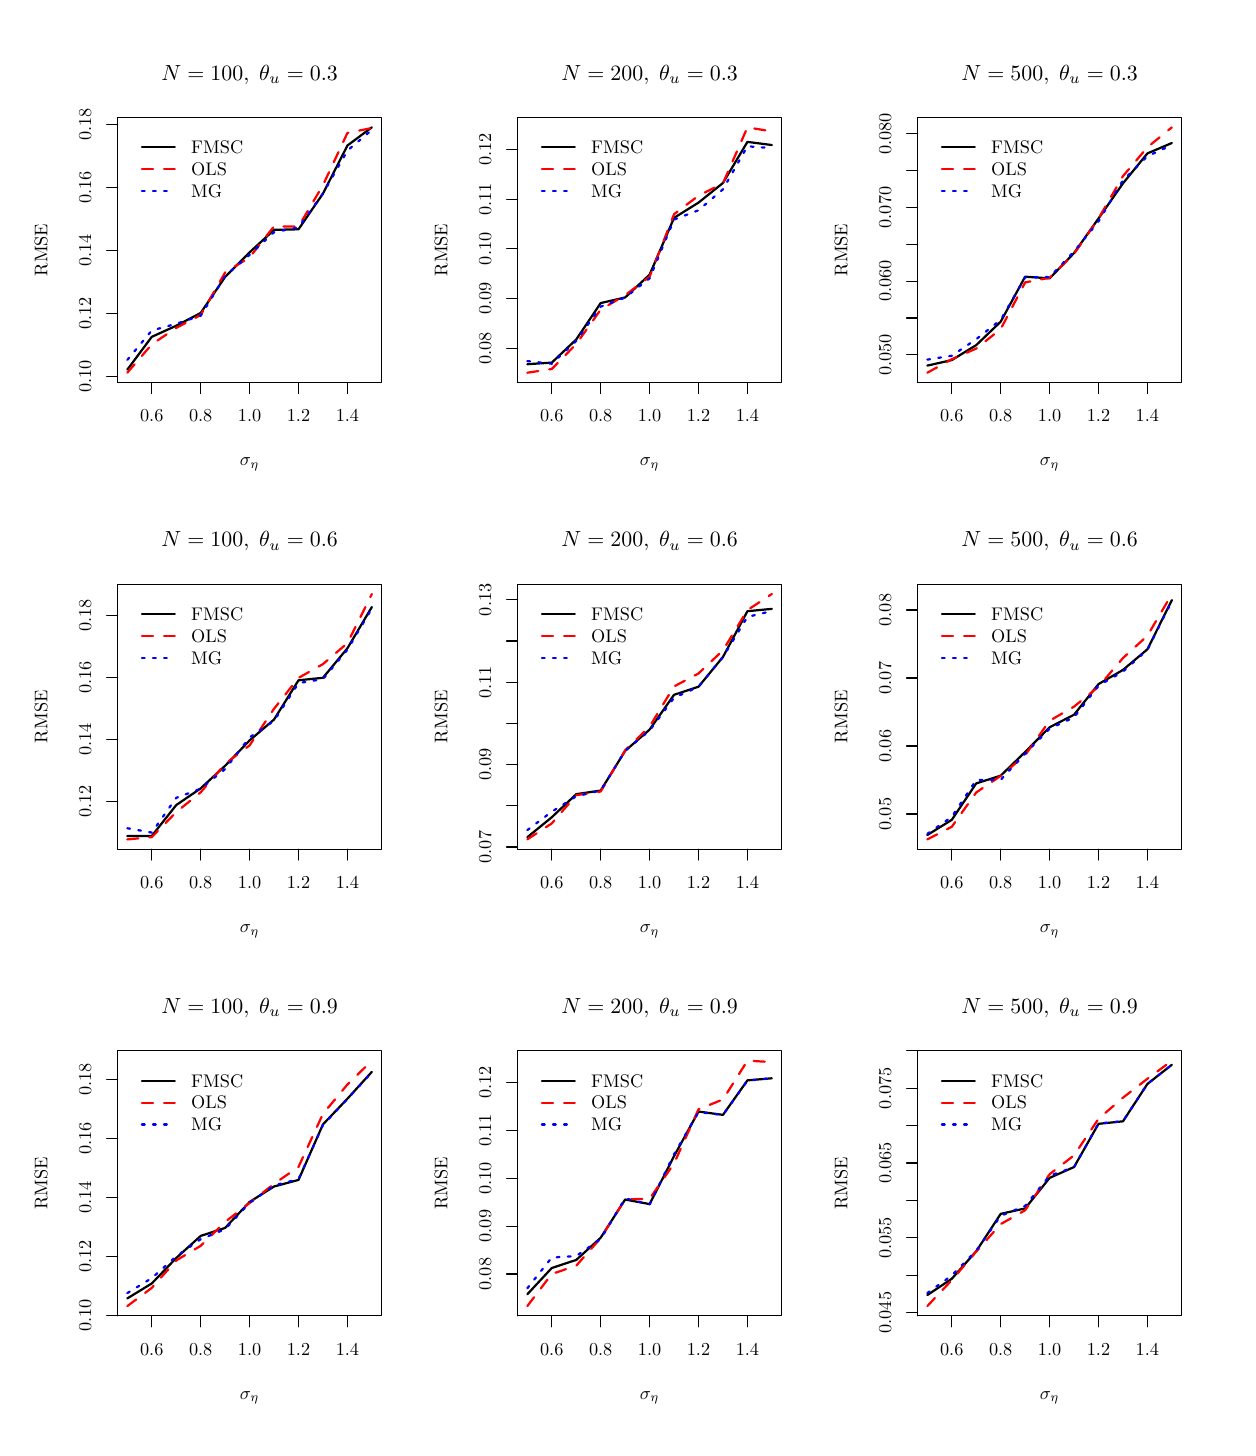
\begin{tikzpicture}[x=1pt,y=1pt]
\definecolor{fillColor}{RGB}{255,255,255}
\path[use as bounding box,fill=fillColor,fill opacity=0.00] (0,0) rectangle (433.62,505.89);
\begin{scope}
\path[clip] ( 32.47,377.65) rectangle (127.91,473.42);
\definecolor{drawColor}{RGB}{0,0,0}

\path[draw=drawColor,line width= 0.8pt,line join=round,line cap=round] ( 36.01,382.32) --
	( 44.84,394.16) --
	( 53.68,398.18) --
	( 62.52,402.80) --
	( 71.35,415.82) --
	( 80.19,424.69) --
	( 89.03,432.84) --
	( 97.86,433.02) --
	(106.70,445.93) --
	(115.54,463.30) --
	(124.37,469.87);
\end{scope}
\begin{scope}
\path[clip] (  0.00,  0.00) rectangle (433.62,505.89);
\definecolor{drawColor}{RGB}{0,0,0}

\path[draw=drawColor,line width= 0.4pt,line join=round,line cap=round] ( 44.84,377.65) -- (115.54,377.65);

\path[draw=drawColor,line width= 0.4pt,line join=round,line cap=round] ( 44.84,377.65) -- ( 44.84,373.69);

\path[draw=drawColor,line width= 0.4pt,line join=round,line cap=round] ( 62.52,377.65) -- ( 62.52,373.69);

\path[draw=drawColor,line width= 0.4pt,line join=round,line cap=round] ( 80.19,377.65) -- ( 80.19,373.69);

\path[draw=drawColor,line width= 0.4pt,line join=round,line cap=round] ( 97.86,377.65) -- ( 97.86,373.69);

\path[draw=drawColor,line width= 0.4pt,line join=round,line cap=round] (115.54,377.65) -- (115.54,373.69);

\node[text=drawColor,anchor=base,inner sep=0pt, outer sep=0pt, scale=  0.66] at ( 44.84,363.40) {0.6};

\node[text=drawColor,anchor=base,inner sep=0pt, outer sep=0pt, scale=  0.66] at ( 62.52,363.40) {0.8};

\node[text=drawColor,anchor=base,inner sep=0pt, outer sep=0pt, scale=  0.66] at ( 80.19,363.40) {1.0};

\node[text=drawColor,anchor=base,inner sep=0pt, outer sep=0pt, scale=  0.66] at ( 97.86,363.40) {1.2};

\node[text=drawColor,anchor=base,inner sep=0pt, outer sep=0pt, scale=  0.66] at (115.54,363.40) {1.4};

\path[draw=drawColor,line width= 0.4pt,line join=round,line cap=round] ( 32.47,379.95) -- ( 32.47,470.83);

\path[draw=drawColor,line width= 0.4pt,line join=round,line cap=round] ( 32.47,379.95) -- ( 28.51,379.95);

\path[draw=drawColor,line width= 0.4pt,line join=round,line cap=round] ( 32.47,402.67) -- ( 28.51,402.67);

\path[draw=drawColor,line width= 0.4pt,line join=round,line cap=round] ( 32.47,425.39) -- ( 28.51,425.39);

\path[draw=drawColor,line width= 0.4pt,line join=round,line cap=round] ( 32.47,448.11) -- ( 28.51,448.11);

\path[draw=drawColor,line width= 0.4pt,line join=round,line cap=round] ( 32.47,470.83) -- ( 28.51,470.83);

\node[text=drawColor,rotate= 90.00,anchor=base,inner sep=0pt, outer sep=0pt, scale=  0.66] at ( 22.97,379.95) {0.10};

\node[text=drawColor,rotate= 90.00,anchor=base,inner sep=0pt, outer sep=0pt, scale=  0.66] at ( 22.97,402.67) {0.12};

\node[text=drawColor,rotate= 90.00,anchor=base,inner sep=0pt, outer sep=0pt, scale=  0.66] at ( 22.97,425.39) {0.14};

\node[text=drawColor,rotate= 90.00,anchor=base,inner sep=0pt, outer sep=0pt, scale=  0.66] at ( 22.97,448.11) {0.16};

\node[text=drawColor,rotate= 90.00,anchor=base,inner sep=0pt, outer sep=0pt, scale=  0.66] at ( 22.97,470.83) {0.18};

\path[draw=drawColor,line width= 0.4pt,line join=round,line cap=round] ( 32.47,377.65) --
	(127.91,377.65) --
	(127.91,473.42) --
	( 32.47,473.42) --
	( 32.47,377.65);
\end{scope}
\begin{scope}
\path[clip] (  0.00,337.26) rectangle (144.54,505.89);
\definecolor{drawColor}{RGB}{0,0,0}

\node[text=drawColor,anchor=base,inner sep=0pt, outer sep=0pt, scale=  0.79] at ( 80.19,486.92) {\bfseries $N=100, \;\theta_u=0.3$};

\node[text=drawColor,anchor=base,inner sep=0pt, outer sep=0pt, scale=  0.66] at ( 80.19,347.56) {$\sigma_\eta$};

\node[text=drawColor,rotate= 90.00,anchor=base,inner sep=0pt, outer sep=0pt, scale=  0.66] at (  7.13,425.53) {RMSE};
\end{scope}
\begin{scope}
\path[clip] ( 32.47,377.65) rectangle (127.91,473.42);
\definecolor{drawColor}{RGB}{255,0,0}

\path[draw=drawColor,line width= 0.8pt,dash pattern=on 4pt off 4pt ,line join=round,line cap=round] ( 36.01,381.20) --
	( 44.84,391.46) --
	( 53.68,397.39) --
	( 62.52,402.04) --
	( 71.35,417.41) --
	( 80.19,422.90) --
	( 89.03,434.11) --
	( 97.86,433.98) --
	(106.70,448.98) --
	(115.54,467.83) --
	(124.37,469.64);
\definecolor{drawColor}{RGB}{0,0,255}

\path[draw=drawColor,line width= 0.8pt,dash pattern=on 1pt off 3pt ,line join=round,line cap=round] ( 36.01,385.83) --
	( 44.84,396.46) --
	( 53.68,398.88) --
	( 62.52,401.78) --
	( 71.35,416.13) --
	( 80.19,423.80) --
	( 89.03,431.98) --
	( 97.86,433.69) --
	(106.70,445.96) --
	(115.54,461.47) --
	(124.37,468.94);
\definecolor{drawColor}{RGB}{0,0,0}

\path[draw=drawColor,line width= 0.8pt,line join=round,line cap=round] ( 41.28,462.63) -- ( 53.16,462.63);
\definecolor{drawColor}{RGB}{255,0,0}

\path[draw=drawColor,line width= 0.8pt,dash pattern=on 4pt off 4pt ,line join=round,line cap=round] ( 41.28,454.71) -- ( 53.16,454.71);
\definecolor{drawColor}{RGB}{0,0,255}

\path[draw=drawColor,line width= 0.8pt,dash pattern=on 1pt off 3pt ,line join=round,line cap=round] ( 41.28,446.79) -- ( 53.16,446.79);
\definecolor{drawColor}{RGB}{0,0,0}

\node[text=drawColor,anchor=base west,inner sep=0pt, outer sep=0pt, scale=  0.66] at ( 59.10,460.35) {FMSC};

\node[text=drawColor,anchor=base west,inner sep=0pt, outer sep=0pt, scale=  0.66] at ( 59.10,452.43) {OLS};

\node[text=drawColor,anchor=base west,inner sep=0pt, outer sep=0pt, scale=  0.66] at ( 59.10,444.51) {MG};
\end{scope}
\begin{scope}
\path[clip] (177.01,377.65) rectangle (272.45,473.42);
\definecolor{drawColor}{RGB}{0,0,0}

\path[draw=drawColor,line width= 0.8pt,line join=round,line cap=round] (180.55,384.28) --
	(189.38,384.85) --
	(198.22,393.22) --
	(207.06,406.37) --
	(215.89,408.40) --
	(224.73,416.63) --
	(233.57,437.17) --
	(242.40,442.66) --
	(251.24,449.77) --
	(260.08,464.61) --
	(268.91,463.48);
\end{scope}
\begin{scope}
\path[clip] (  0.00,  0.00) rectangle (433.62,505.89);
\definecolor{drawColor}{RGB}{0,0,0}

\path[draw=drawColor,line width= 0.4pt,line join=round,line cap=round] (189.38,377.65) -- (260.08,377.65);

\path[draw=drawColor,line width= 0.4pt,line join=round,line cap=round] (189.38,377.65) -- (189.38,373.69);

\path[draw=drawColor,line width= 0.4pt,line join=round,line cap=round] (207.06,377.65) -- (207.06,373.69);

\path[draw=drawColor,line width= 0.4pt,line join=round,line cap=round] (224.73,377.65) -- (224.73,373.69);

\path[draw=drawColor,line width= 0.4pt,line join=round,line cap=round] (242.40,377.65) -- (242.40,373.69);

\path[draw=drawColor,line width= 0.4pt,line join=round,line cap=round] (260.08,377.65) -- (260.08,373.69);

\node[text=drawColor,anchor=base,inner sep=0pt, outer sep=0pt, scale=  0.66] at (189.38,363.40) {0.6};

\node[text=drawColor,anchor=base,inner sep=0pt, outer sep=0pt, scale=  0.66] at (207.06,363.40) {0.8};

\node[text=drawColor,anchor=base,inner sep=0pt, outer sep=0pt, scale=  0.66] at (224.73,363.40) {1.0};

\node[text=drawColor,anchor=base,inner sep=0pt, outer sep=0pt, scale=  0.66] at (242.40,363.40) {1.2};

\node[text=drawColor,anchor=base,inner sep=0pt, outer sep=0pt, scale=  0.66] at (260.08,363.40) {1.4};

\path[draw=drawColor,line width= 0.4pt,line join=round,line cap=round] (177.01,390.07) -- (177.01,461.88);

\path[draw=drawColor,line width= 0.4pt,line join=round,line cap=round] (177.01,390.07) -- (173.05,390.07);

\path[draw=drawColor,line width= 0.4pt,line join=round,line cap=round] (177.01,408.02) -- (173.05,408.02);

\path[draw=drawColor,line width= 0.4pt,line join=round,line cap=round] (177.01,425.97) -- (173.05,425.97);

\path[draw=drawColor,line width= 0.4pt,line join=round,line cap=round] (177.01,443.92) -- (173.05,443.92);

\path[draw=drawColor,line width= 0.4pt,line join=round,line cap=round] (177.01,461.88) -- (173.05,461.88);

\node[text=drawColor,rotate= 90.00,anchor=base,inner sep=0pt, outer sep=0pt, scale=  0.66] at (167.51,390.07) {0.08};

\node[text=drawColor,rotate= 90.00,anchor=base,inner sep=0pt, outer sep=0pt, scale=  0.66] at (167.51,408.02) {0.09};

\node[text=drawColor,rotate= 90.00,anchor=base,inner sep=0pt, outer sep=0pt, scale=  0.66] at (167.51,425.97) {0.10};

\node[text=drawColor,rotate= 90.00,anchor=base,inner sep=0pt, outer sep=0pt, scale=  0.66] at (167.51,443.92) {0.11};

\node[text=drawColor,rotate= 90.00,anchor=base,inner sep=0pt, outer sep=0pt, scale=  0.66] at (167.51,461.88) {0.12};

\path[draw=drawColor,line width= 0.4pt,line join=round,line cap=round] (177.01,377.65) --
	(272.45,377.65) --
	(272.45,473.42) --
	(177.01,473.42) --
	(177.01,377.65);
\end{scope}
\begin{scope}
\path[clip] (144.54,337.26) rectangle (289.08,505.89);
\definecolor{drawColor}{RGB}{0,0,0}

\node[text=drawColor,anchor=base,inner sep=0pt, outer sep=0pt, scale=  0.79] at (224.73,486.92) {\bfseries $N=200, \;\theta_u=0.3$};

\node[text=drawColor,anchor=base,inner sep=0pt, outer sep=0pt, scale=  0.66] at (224.73,347.56) {$\sigma_\eta$};

\node[text=drawColor,rotate= 90.00,anchor=base,inner sep=0pt, outer sep=0pt, scale=  0.66] at (151.67,425.53) {RMSE};
\end{scope}
\begin{scope}
\path[clip] (177.01,377.65) rectangle (272.45,473.42);
\definecolor{drawColor}{RGB}{255,0,0}

\path[draw=drawColor,line width= 0.8pt,dash pattern=on 4pt off 4pt ,line join=round,line cap=round] (180.55,381.20) --
	(189.38,382.54) --
	(198.22,391.56) --
	(207.06,404.00) --
	(215.89,409.22) --
	(224.73,415.90) --
	(233.57,438.48) --
	(242.40,445.16) --
	(251.24,449.64) --
	(260.08,469.87) --
	(268.91,468.40);
\definecolor{drawColor}{RGB}{0,0,255}

\path[draw=drawColor,line width= 0.8pt,dash pattern=on 1pt off 3pt ,line join=round,line cap=round] (180.55,385.40) --
	(189.38,384.46) --
	(198.22,392.68) --
	(207.06,405.08) --
	(215.89,408.37) --
	(224.73,415.30) --
	(233.57,436.54) --
	(242.40,439.90) --
	(251.24,447.48) --
	(260.08,463.02) --
	(268.91,462.36);
\definecolor{drawColor}{RGB}{0,0,0}

\path[draw=drawColor,line width= 0.8pt,line join=round,line cap=round] (185.82,462.63) -- (197.70,462.63);
\definecolor{drawColor}{RGB}{255,0,0}

\path[draw=drawColor,line width= 0.8pt,dash pattern=on 4pt off 4pt ,line join=round,line cap=round] (185.82,454.71) -- (197.70,454.71);
\definecolor{drawColor}{RGB}{0,0,255}

\path[draw=drawColor,line width= 0.8pt,dash pattern=on 1pt off 3pt ,line join=round,line cap=round] (185.82,446.79) -- (197.70,446.79);
\definecolor{drawColor}{RGB}{0,0,0}

\node[text=drawColor,anchor=base west,inner sep=0pt, outer sep=0pt, scale=  0.66] at (203.64,460.35) {FMSC};

\node[text=drawColor,anchor=base west,inner sep=0pt, outer sep=0pt, scale=  0.66] at (203.64,452.43) {OLS};

\node[text=drawColor,anchor=base west,inner sep=0pt, outer sep=0pt, scale=  0.66] at (203.64,444.51) {MG};
\end{scope}
\begin{scope}
\path[clip] (321.55,377.65) rectangle (416.99,473.42);
\definecolor{drawColor}{RGB}{0,0,0}

\path[draw=drawColor,line width= 0.8pt,line join=round,line cap=round] (325.09,383.77) --
	(333.92,385.76) --
	(342.76,391.18) --
	(351.60,399.65) --
	(360.43,415.90) --
	(369.27,415.30) --
	(378.11,424.45) --
	(386.94,436.94) --
	(395.78,449.63) --
	(404.62,460.45) --
	(413.45,464.21);
\end{scope}
\begin{scope}
\path[clip] (  0.00,  0.00) rectangle (433.62,505.89);
\definecolor{drawColor}{RGB}{0,0,0}

\path[draw=drawColor,line width= 0.4pt,line join=round,line cap=round] (333.92,377.65) -- (404.62,377.65);

\path[draw=drawColor,line width= 0.4pt,line join=round,line cap=round] (333.92,377.65) -- (333.92,373.69);

\path[draw=drawColor,line width= 0.4pt,line join=round,line cap=round] (351.60,377.65) -- (351.60,373.69);

\path[draw=drawColor,line width= 0.4pt,line join=round,line cap=round] (369.27,377.65) -- (369.27,373.69);

\path[draw=drawColor,line width= 0.4pt,line join=round,line cap=round] (386.94,377.65) -- (386.94,373.69);

\path[draw=drawColor,line width= 0.4pt,line join=round,line cap=round] (404.62,377.65) -- (404.62,373.69);

\node[text=drawColor,anchor=base,inner sep=0pt, outer sep=0pt, scale=  0.66] at (333.92,363.40) {0.6};

\node[text=drawColor,anchor=base,inner sep=0pt, outer sep=0pt, scale=  0.66] at (351.60,363.40) {0.8};

\node[text=drawColor,anchor=base,inner sep=0pt, outer sep=0pt, scale=  0.66] at (369.27,363.40) {1.0};

\node[text=drawColor,anchor=base,inner sep=0pt, outer sep=0pt, scale=  0.66] at (386.94,363.40) {1.2};

\node[text=drawColor,anchor=base,inner sep=0pt, outer sep=0pt, scale=  0.66] at (404.62,363.40) {1.4};

\path[draw=drawColor,line width= 0.4pt,line join=round,line cap=round] (321.55,387.68) -- (321.55,467.50);

\path[draw=drawColor,line width= 0.4pt,line join=round,line cap=round] (321.55,387.68) -- (317.59,387.68);

\path[draw=drawColor,line width= 0.4pt,line join=round,line cap=round] (321.55,400.99) -- (317.59,400.99);

\path[draw=drawColor,line width= 0.4pt,line join=round,line cap=round] (321.55,414.29) -- (317.59,414.29);

\path[draw=drawColor,line width= 0.4pt,line join=round,line cap=round] (321.55,427.59) -- (317.59,427.59);

\path[draw=drawColor,line width= 0.4pt,line join=round,line cap=round] (321.55,440.90) -- (317.59,440.90);

\path[draw=drawColor,line width= 0.4pt,line join=round,line cap=round] (321.55,454.20) -- (317.59,454.20);

\path[draw=drawColor,line width= 0.4pt,line join=round,line cap=round] (321.55,467.50) -- (317.59,467.50);

\node[text=drawColor,rotate= 90.00,anchor=base,inner sep=0pt, outer sep=0pt, scale=  0.66] at (312.05,387.68) {0.050};

\node[text=drawColor,rotate= 90.00,anchor=base,inner sep=0pt, outer sep=0pt, scale=  0.66] at (312.05,414.29) {0.060};

\node[text=drawColor,rotate= 90.00,anchor=base,inner sep=0pt, outer sep=0pt, scale=  0.66] at (312.05,440.90) {0.070};

\node[text=drawColor,rotate= 90.00,anchor=base,inner sep=0pt, outer sep=0pt, scale=  0.66] at (312.05,467.50) {0.080};

\path[draw=drawColor,line width= 0.4pt,line join=round,line cap=round] (321.55,377.65) --
	(416.99,377.65) --
	(416.99,473.42) --
	(321.55,473.42) --
	(321.55,377.65);
\end{scope}
\begin{scope}
\path[clip] (289.08,337.26) rectangle (433.62,505.89);
\definecolor{drawColor}{RGB}{0,0,0}

\node[text=drawColor,anchor=base,inner sep=0pt, outer sep=0pt, scale=  0.79] at (369.27,486.92) {\bfseries $N=500, \;\theta_u=0.3$};

\node[text=drawColor,anchor=base,inner sep=0pt, outer sep=0pt, scale=  0.66] at (369.27,347.56) {$\sigma_\eta$};

\node[text=drawColor,rotate= 90.00,anchor=base,inner sep=0pt, outer sep=0pt, scale=  0.66] at (296.21,425.53) {RMSE};
\end{scope}
\begin{scope}
\path[clip] (321.55,377.65) rectangle (416.99,473.42);
\definecolor{drawColor}{RGB}{255,0,0}

\path[draw=drawColor,line width= 0.8pt,dash pattern=on 4pt off 4pt ,line join=round,line cap=round] (325.09,381.20) --
	(333.92,386.09) --
	(342.76,389.94) --
	(351.60,396.98) --
	(360.43,413.84) --
	(369.27,415.51) --
	(378.11,424.15) --
	(386.94,436.90) --
	(395.78,452.24) --
	(404.62,462.68) --
	(413.45,469.87);
\definecolor{drawColor}{RGB}{0,0,255}

\path[draw=drawColor,line width= 0.8pt,dash pattern=on 1pt off 3pt ,line join=round,line cap=round] (325.09,385.94) --
	(333.92,387.34) --
	(342.76,393.32) --
	(351.60,400.29) --
	(360.43,415.67) --
	(369.27,415.77) --
	(378.11,425.00) --
	(386.94,435.88) --
	(395.78,450.73) --
	(404.62,459.45) --
	(413.45,463.47);
\definecolor{drawColor}{RGB}{0,0,0}

\path[draw=drawColor,line width= 0.8pt,line join=round,line cap=round] (330.36,462.63) -- (342.24,462.63);
\definecolor{drawColor}{RGB}{255,0,0}

\path[draw=drawColor,line width= 0.8pt,dash pattern=on 4pt off 4pt ,line join=round,line cap=round] (330.36,454.71) -- (342.24,454.71);
\definecolor{drawColor}{RGB}{0,0,255}

\path[draw=drawColor,line width= 0.8pt,dash pattern=on 1pt off 3pt ,line join=round,line cap=round] (330.36,446.79) -- (342.24,446.79);
\definecolor{drawColor}{RGB}{0,0,0}

\node[text=drawColor,anchor=base west,inner sep=0pt, outer sep=0pt, scale=  0.66] at (348.18,460.35) {FMSC};

\node[text=drawColor,anchor=base west,inner sep=0pt, outer sep=0pt, scale=  0.66] at (348.18,452.43) {OLS};

\node[text=drawColor,anchor=base west,inner sep=0pt, outer sep=0pt, scale=  0.66] at (348.18,444.51) {MG};
\end{scope}
\begin{scope}
\path[clip] ( 32.47,209.02) rectangle (127.91,304.79);
\definecolor{drawColor}{RGB}{0,0,0}

\path[draw=drawColor,line width= 0.8pt,line join=round,line cap=round] ( 36.01,213.79) --
	( 44.84,213.81) --
	( 53.68,224.97) --
	( 62.52,231.01) --
	( 71.35,239.18) --
	( 80.19,248.33) --
	( 89.03,255.90) --
	( 97.86,270.06) --
	(106.70,270.97) --
	(115.54,281.64) --
	(124.37,296.55);
\end{scope}
\begin{scope}
\path[clip] (  0.00,  0.00) rectangle (433.62,505.89);
\definecolor{drawColor}{RGB}{0,0,0}

\path[draw=drawColor,line width= 0.4pt,line join=round,line cap=round] ( 44.84,209.02) -- (115.54,209.02);

\path[draw=drawColor,line width= 0.4pt,line join=round,line cap=round] ( 44.84,209.02) -- ( 44.84,205.06);

\path[draw=drawColor,line width= 0.4pt,line join=round,line cap=round] ( 62.52,209.02) -- ( 62.52,205.06);

\path[draw=drawColor,line width= 0.4pt,line join=round,line cap=round] ( 80.19,209.02) -- ( 80.19,205.06);

\path[draw=drawColor,line width= 0.4pt,line join=round,line cap=round] ( 97.86,209.02) -- ( 97.86,205.06);

\path[draw=drawColor,line width= 0.4pt,line join=round,line cap=round] (115.54,209.02) -- (115.54,205.06);

\node[text=drawColor,anchor=base,inner sep=0pt, outer sep=0pt, scale=  0.66] at ( 44.84,194.77) {0.6};

\node[text=drawColor,anchor=base,inner sep=0pt, outer sep=0pt, scale=  0.66] at ( 62.52,194.77) {0.8};

\node[text=drawColor,anchor=base,inner sep=0pt, outer sep=0pt, scale=  0.66] at ( 80.19,194.77) {1.0};

\node[text=drawColor,anchor=base,inner sep=0pt, outer sep=0pt, scale=  0.66] at ( 97.86,194.77) {1.2};

\node[text=drawColor,anchor=base,inner sep=0pt, outer sep=0pt, scale=  0.66] at (115.54,194.77) {1.4};

\path[draw=drawColor,line width= 0.4pt,line join=round,line cap=round] ( 32.47,226.39) -- ( 32.47,293.50);

\path[draw=drawColor,line width= 0.4pt,line join=round,line cap=round] ( 32.47,226.39) -- ( 28.51,226.39);

\path[draw=drawColor,line width= 0.4pt,line join=round,line cap=round] ( 32.47,248.76) -- ( 28.51,248.76);

\path[draw=drawColor,line width= 0.4pt,line join=round,line cap=round] ( 32.47,271.13) -- ( 28.51,271.13);

\path[draw=drawColor,line width= 0.4pt,line join=round,line cap=round] ( 32.47,293.50) -- ( 28.51,293.50);

\node[text=drawColor,rotate= 90.00,anchor=base,inner sep=0pt, outer sep=0pt, scale=  0.66] at ( 22.97,226.39) {0.12};

\node[text=drawColor,rotate= 90.00,anchor=base,inner sep=0pt, outer sep=0pt, scale=  0.66] at ( 22.97,248.76) {0.14};

\node[text=drawColor,rotate= 90.00,anchor=base,inner sep=0pt, outer sep=0pt, scale=  0.66] at ( 22.97,271.13) {0.16};

\node[text=drawColor,rotate= 90.00,anchor=base,inner sep=0pt, outer sep=0pt, scale=  0.66] at ( 22.97,293.50) {0.18};

\path[draw=drawColor,line width= 0.4pt,line join=round,line cap=round] ( 32.47,209.02) --
	(127.91,209.02) --
	(127.91,304.79) --
	( 32.47,304.79) --
	( 32.47,209.02);
\end{scope}
\begin{scope}
\path[clip] (  0.00,168.63) rectangle (144.54,337.26);
\definecolor{drawColor}{RGB}{0,0,0}

\node[text=drawColor,anchor=base,inner sep=0pt, outer sep=0pt, scale=  0.79] at ( 80.19,318.29) {\bfseries $N=100, \;\theta_u=0.6$};

\node[text=drawColor,anchor=base,inner sep=0pt, outer sep=0pt, scale=  0.66] at ( 80.19,178.93) {$\sigma_\eta$};

\node[text=drawColor,rotate= 90.00,anchor=base,inner sep=0pt, outer sep=0pt, scale=  0.66] at (  7.13,256.90) {RMSE};
\end{scope}
\begin{scope}
\path[clip] ( 32.47,209.02) rectangle (127.91,304.79);
\definecolor{drawColor}{RGB}{255,0,0}

\path[draw=drawColor,line width= 0.8pt,dash pattern=on 4pt off 4pt ,line join=round,line cap=round] ( 36.01,212.57) --
	( 44.84,213.39) --
	( 53.68,222.43) --
	( 62.52,229.59) --
	( 71.35,239.85) --
	( 80.19,246.54) --
	( 89.03,259.78) --
	( 97.86,270.92) --
	(106.70,275.91) --
	(115.54,283.50) --
	(124.37,301.24);
\definecolor{drawColor}{RGB}{0,0,255}

\path[draw=drawColor,line width= 0.8pt,dash pattern=on 1pt off 3pt ,line join=round,line cap=round] ( 36.01,216.61) --
	( 44.84,215.03) --
	( 53.68,227.58) --
	( 62.52,230.89) --
	( 71.35,237.98) --
	( 80.19,249.43) --
	( 89.03,255.41) --
	( 97.86,269.06) --
	(106.70,270.47) --
	(115.54,281.13) --
	(124.37,296.02);
\definecolor{drawColor}{RGB}{0,0,0}

\path[draw=drawColor,line width= 0.8pt,line join=round,line cap=round] ( 41.28,294.00) -- ( 53.16,294.00);
\definecolor{drawColor}{RGB}{255,0,0}

\path[draw=drawColor,line width= 0.8pt,dash pattern=on 4pt off 4pt ,line join=round,line cap=round] ( 41.28,286.08) -- ( 53.16,286.08);
\definecolor{drawColor}{RGB}{0,0,255}

\path[draw=drawColor,line width= 0.8pt,dash pattern=on 1pt off 3pt ,line join=round,line cap=round] ( 41.28,278.16) -- ( 53.16,278.16);
\definecolor{drawColor}{RGB}{0,0,0}

\node[text=drawColor,anchor=base west,inner sep=0pt, outer sep=0pt, scale=  0.66] at ( 59.10,291.72) {FMSC};

\node[text=drawColor,anchor=base west,inner sep=0pt, outer sep=0pt, scale=  0.66] at ( 59.10,283.80) {OLS};

\node[text=drawColor,anchor=base west,inner sep=0pt, outer sep=0pt, scale=  0.66] at ( 59.10,275.88) {MG};
\end{scope}
\begin{scope}
\path[clip] (177.01,209.02) rectangle (272.45,304.79);
\definecolor{drawColor}{RGB}{0,0,0}

\path[draw=drawColor,line width= 0.8pt,line join=round,line cap=round] (180.55,213.36) --
	(189.38,220.57) --
	(198.22,228.92) --
	(207.06,230.23) --
	(215.89,244.56) --
	(224.73,252.25) --
	(233.57,264.82) --
	(242.40,267.73) --
	(251.24,278.49) --
	(260.08,295.03) --
	(268.91,295.87);
\end{scope}
\begin{scope}
\path[clip] (  0.00,  0.00) rectangle (433.62,505.89);
\definecolor{drawColor}{RGB}{0,0,0}

\path[draw=drawColor,line width= 0.4pt,line join=round,line cap=round] (189.38,209.02) -- (260.08,209.02);

\path[draw=drawColor,line width= 0.4pt,line join=round,line cap=round] (189.38,209.02) -- (189.38,205.06);

\path[draw=drawColor,line width= 0.4pt,line join=round,line cap=round] (207.06,209.02) -- (207.06,205.06);

\path[draw=drawColor,line width= 0.4pt,line join=round,line cap=round] (224.73,209.02) -- (224.73,205.06);

\path[draw=drawColor,line width= 0.4pt,line join=round,line cap=round] (242.40,209.02) -- (242.40,205.06);

\path[draw=drawColor,line width= 0.4pt,line join=round,line cap=round] (260.08,209.02) -- (260.08,205.06);

\node[text=drawColor,anchor=base,inner sep=0pt, outer sep=0pt, scale=  0.66] at (189.38,194.77) {0.6};

\node[text=drawColor,anchor=base,inner sep=0pt, outer sep=0pt, scale=  0.66] at (207.06,194.77) {0.8};

\node[text=drawColor,anchor=base,inner sep=0pt, outer sep=0pt, scale=  0.66] at (224.73,194.77) {1.0};

\node[text=drawColor,anchor=base,inner sep=0pt, outer sep=0pt, scale=  0.66] at (242.40,194.77) {1.2};

\node[text=drawColor,anchor=base,inner sep=0pt, outer sep=0pt, scale=  0.66] at (260.08,194.77) {1.4};

\path[draw=drawColor,line width= 0.4pt,line join=round,line cap=round] (177.01,209.82) -- (177.01,299.13);

\path[draw=drawColor,line width= 0.4pt,line join=round,line cap=round] (177.01,209.82) -- (173.05,209.82);

\path[draw=drawColor,line width= 0.4pt,line join=round,line cap=round] (177.01,224.70) -- (173.05,224.70);

\path[draw=drawColor,line width= 0.4pt,line join=round,line cap=round] (177.01,239.59) -- (173.05,239.59);

\path[draw=drawColor,line width= 0.4pt,line join=round,line cap=round] (177.01,254.48) -- (173.05,254.48);

\path[draw=drawColor,line width= 0.4pt,line join=round,line cap=round] (177.01,269.36) -- (173.05,269.36);

\path[draw=drawColor,line width= 0.4pt,line join=round,line cap=round] (177.01,284.25) -- (173.05,284.25);

\path[draw=drawColor,line width= 0.4pt,line join=round,line cap=round] (177.01,299.13) -- (173.05,299.13);

\node[text=drawColor,rotate= 90.00,anchor=base,inner sep=0pt, outer sep=0pt, scale=  0.66] at (167.51,209.82) {0.07};

\node[text=drawColor,rotate= 90.00,anchor=base,inner sep=0pt, outer sep=0pt, scale=  0.66] at (167.51,239.59) {0.09};

\node[text=drawColor,rotate= 90.00,anchor=base,inner sep=0pt, outer sep=0pt, scale=  0.66] at (167.51,269.36) {0.11};

\node[text=drawColor,rotate= 90.00,anchor=base,inner sep=0pt, outer sep=0pt, scale=  0.66] at (167.51,299.13) {0.13};

\path[draw=drawColor,line width= 0.4pt,line join=round,line cap=round] (177.01,209.02) --
	(272.45,209.02) --
	(272.45,304.79) --
	(177.01,304.79) --
	(177.01,209.02);
\end{scope}
\begin{scope}
\path[clip] (144.54,168.63) rectangle (289.08,337.26);
\definecolor{drawColor}{RGB}{0,0,0}

\node[text=drawColor,anchor=base,inner sep=0pt, outer sep=0pt, scale=  0.79] at (224.73,318.29) {\bfseries $N=200, \;\theta_u=0.6$};

\node[text=drawColor,anchor=base,inner sep=0pt, outer sep=0pt, scale=  0.66] at (224.73,178.93) {$\sigma_\eta$};

\node[text=drawColor,rotate= 90.00,anchor=base,inner sep=0pt, outer sep=0pt, scale=  0.66] at (151.67,256.90) {RMSE};
\end{scope}
\begin{scope}
\path[clip] (177.01,209.02) rectangle (272.45,304.79);
\definecolor{drawColor}{RGB}{255,0,0}

\path[draw=drawColor,line width= 0.8pt,dash pattern=on 4pt off 4pt ,line join=round,line cap=round] (180.55,212.57) --
	(189.38,218.34) --
	(198.22,228.54) --
	(207.06,229.87) --
	(215.89,244.75) --
	(224.73,253.33) --
	(233.57,267.85) --
	(242.40,272.53) --
	(251.24,280.89) --
	(260.08,295.43) --
	(268.91,301.24);
\definecolor{drawColor}{RGB}{0,0,255}

\path[draw=drawColor,line width= 0.8pt,dash pattern=on 1pt off 3pt ,line join=round,line cap=round] (180.55,215.94) --
	(189.38,222.58) --
	(198.22,228.14) --
	(207.06,230.25) --
	(215.89,244.58) --
	(224.73,251.91) --
	(233.57,263.74) --
	(242.40,267.71) --
	(251.24,278.47) --
	(260.08,292.98) --
	(268.91,295.08);
\definecolor{drawColor}{RGB}{0,0,0}

\path[draw=drawColor,line width= 0.8pt,line join=round,line cap=round] (185.82,294.00) -- (197.70,294.00);
\definecolor{drawColor}{RGB}{255,0,0}

\path[draw=drawColor,line width= 0.8pt,dash pattern=on 4pt off 4pt ,line join=round,line cap=round] (185.82,286.08) -- (197.70,286.08);
\definecolor{drawColor}{RGB}{0,0,255}

\path[draw=drawColor,line width= 0.8pt,dash pattern=on 1pt off 3pt ,line join=round,line cap=round] (185.82,278.16) -- (197.70,278.16);
\definecolor{drawColor}{RGB}{0,0,0}

\node[text=drawColor,anchor=base west,inner sep=0pt, outer sep=0pt, scale=  0.66] at (203.64,291.72) {FMSC};

\node[text=drawColor,anchor=base west,inner sep=0pt, outer sep=0pt, scale=  0.66] at (203.64,283.80) {OLS};

\node[text=drawColor,anchor=base west,inner sep=0pt, outer sep=0pt, scale=  0.66] at (203.64,275.88) {MG};
\end{scope}
\begin{scope}
\path[clip] (321.55,209.02) rectangle (416.99,304.79);
\definecolor{drawColor}{RGB}{0,0,0}

\path[draw=drawColor,line width= 0.8pt,line join=round,line cap=round] (325.09,214.15) --
	(333.92,219.64) --
	(342.76,232.81) --
	(351.60,235.60) --
	(360.43,244.16) --
	(369.27,253.09) --
	(378.11,257.63) --
	(386.94,268.69) --
	(395.78,273.81) --
	(404.62,281.27) --
	(413.45,299.05);
\end{scope}
\begin{scope}
\path[clip] (  0.00,  0.00) rectangle (433.62,505.89);
\definecolor{drawColor}{RGB}{0,0,0}

\path[draw=drawColor,line width= 0.4pt,line join=round,line cap=round] (333.92,209.02) -- (404.62,209.02);

\path[draw=drawColor,line width= 0.4pt,line join=round,line cap=round] (333.92,209.02) -- (333.92,205.06);

\path[draw=drawColor,line width= 0.4pt,line join=round,line cap=round] (351.60,209.02) -- (351.60,205.06);

\path[draw=drawColor,line width= 0.4pt,line join=round,line cap=round] (369.27,209.02) -- (369.27,205.06);

\path[draw=drawColor,line width= 0.4pt,line join=round,line cap=round] (386.94,209.02) -- (386.94,205.06);

\path[draw=drawColor,line width= 0.4pt,line join=round,line cap=round] (404.62,209.02) -- (404.62,205.06);

\node[text=drawColor,anchor=base,inner sep=0pt, outer sep=0pt, scale=  0.66] at (333.92,194.77) {0.6};

\node[text=drawColor,anchor=base,inner sep=0pt, outer sep=0pt, scale=  0.66] at (351.60,194.77) {0.8};

\node[text=drawColor,anchor=base,inner sep=0pt, outer sep=0pt, scale=  0.66] at (369.27,194.77) {1.0};

\node[text=drawColor,anchor=base,inner sep=0pt, outer sep=0pt, scale=  0.66] at (386.94,194.77) {1.2};

\node[text=drawColor,anchor=base,inner sep=0pt, outer sep=0pt, scale=  0.66] at (404.62,194.77) {1.4};

\path[draw=drawColor,line width= 0.4pt,line join=round,line cap=round] (321.55,221.75) -- (321.55,295.45);

\path[draw=drawColor,line width= 0.4pt,line join=round,line cap=round] (321.55,221.75) -- (317.59,221.75);

\path[draw=drawColor,line width= 0.4pt,line join=round,line cap=round] (321.55,246.31) -- (317.59,246.31);

\path[draw=drawColor,line width= 0.4pt,line join=round,line cap=round] (321.55,270.88) -- (317.59,270.88);

\path[draw=drawColor,line width= 0.4pt,line join=round,line cap=round] (321.55,295.45) -- (317.59,295.45);

\node[text=drawColor,rotate= 90.00,anchor=base,inner sep=0pt, outer sep=0pt, scale=  0.66] at (312.05,221.75) {0.05};

\node[text=drawColor,rotate= 90.00,anchor=base,inner sep=0pt, outer sep=0pt, scale=  0.66] at (312.05,246.31) {0.06};

\node[text=drawColor,rotate= 90.00,anchor=base,inner sep=0pt, outer sep=0pt, scale=  0.66] at (312.05,270.88) {0.07};

\node[text=drawColor,rotate= 90.00,anchor=base,inner sep=0pt, outer sep=0pt, scale=  0.66] at (312.05,295.45) {0.08};

\path[draw=drawColor,line width= 0.4pt,line join=round,line cap=round] (321.55,209.02) --
	(416.99,209.02) --
	(416.99,304.79) --
	(321.55,304.79) --
	(321.55,209.02);
\end{scope}
\begin{scope}
\path[clip] (289.08,168.63) rectangle (433.62,337.26);
\definecolor{drawColor}{RGB}{0,0,0}

\node[text=drawColor,anchor=base,inner sep=0pt, outer sep=0pt, scale=  0.79] at (369.27,318.29) {\bfseries $N=500, \;\theta_u=0.6$};

\node[text=drawColor,anchor=base,inner sep=0pt, outer sep=0pt, scale=  0.66] at (369.27,178.93) {$\sigma_\eta$};

\node[text=drawColor,rotate= 90.00,anchor=base,inner sep=0pt, outer sep=0pt, scale=  0.66] at (296.21,256.90) {RMSE};
\end{scope}
\begin{scope}
\path[clip] (321.55,209.02) rectangle (416.99,304.79);
\definecolor{drawColor}{RGB}{255,0,0}

\path[draw=drawColor,line width= 0.8pt,dash pattern=on 4pt off 4pt ,line join=round,line cap=round] (325.09,212.57) --
	(333.92,217.13) --
	(342.76,229.53) --
	(351.60,235.51) --
	(360.43,242.99) --
	(369.27,255.45) --
	(378.11,260.55) --
	(386.94,267.77) --
	(395.78,278.10) --
	(404.62,286.16) --
	(413.45,301.24);
\definecolor{drawColor}{RGB}{0,0,255}

\path[draw=drawColor,line width= 0.8pt,dash pattern=on 1pt off 3pt ,line join=round,line cap=round] (325.09,214.57) --
	(333.92,220.71) --
	(342.76,234.06) --
	(351.60,234.10) --
	(360.43,243.53) --
	(369.27,252.60) --
	(378.11,256.67) --
	(386.94,268.15) --
	(395.78,273.18) --
	(404.62,281.10) --
	(413.45,298.68);
\definecolor{drawColor}{RGB}{0,0,0}

\path[draw=drawColor,line width= 0.8pt,line join=round,line cap=round] (330.36,294.00) -- (342.24,294.00);
\definecolor{drawColor}{RGB}{255,0,0}

\path[draw=drawColor,line width= 0.8pt,dash pattern=on 4pt off 4pt ,line join=round,line cap=round] (330.36,286.08) -- (342.24,286.08);
\definecolor{drawColor}{RGB}{0,0,255}

\path[draw=drawColor,line width= 0.8pt,dash pattern=on 1pt off 3pt ,line join=round,line cap=round] (330.36,278.16) -- (342.24,278.16);
\definecolor{drawColor}{RGB}{0,0,0}

\node[text=drawColor,anchor=base west,inner sep=0pt, outer sep=0pt, scale=  0.66] at (348.18,291.72) {FMSC};

\node[text=drawColor,anchor=base west,inner sep=0pt, outer sep=0pt, scale=  0.66] at (348.18,283.80) {OLS};

\node[text=drawColor,anchor=base west,inner sep=0pt, outer sep=0pt, scale=  0.66] at (348.18,275.88) {MG};
\end{scope}
\begin{scope}
\path[clip] ( 32.47, 40.39) rectangle (127.91,136.16);
\definecolor{drawColor}{RGB}{0,0,0}

\path[draw=drawColor,line width= 0.8pt,line join=round,line cap=round] ( 36.01, 46.71) --
	( 44.84, 52.11) --
	( 53.68, 61.31) --
	( 62.52, 69.29) --
	( 71.35, 72.19) --
	( 80.19, 81.57) --
	( 89.03, 87.15) --
	( 97.86, 89.52) --
	(106.70,109.59) --
	(115.54,118.86) --
	(124.37,128.58);
\end{scope}
\begin{scope}
\path[clip] (  0.00,  0.00) rectangle (433.62,505.89);
\definecolor{drawColor}{RGB}{0,0,0}

\path[draw=drawColor,line width= 0.4pt,line join=round,line cap=round] ( 44.84, 40.39) -- (115.54, 40.39);

\path[draw=drawColor,line width= 0.4pt,line join=round,line cap=round] ( 44.84, 40.39) -- ( 44.84, 36.43);

\path[draw=drawColor,line width= 0.4pt,line join=round,line cap=round] ( 62.52, 40.39) -- ( 62.52, 36.43);

\path[draw=drawColor,line width= 0.4pt,line join=round,line cap=round] ( 80.19, 40.39) -- ( 80.19, 36.43);

\path[draw=drawColor,line width= 0.4pt,line join=round,line cap=round] ( 97.86, 40.39) -- ( 97.86, 36.43);

\path[draw=drawColor,line width= 0.4pt,line join=round,line cap=round] (115.54, 40.39) -- (115.54, 36.43);

\node[text=drawColor,anchor=base,inner sep=0pt, outer sep=0pt, scale=  0.66] at ( 44.84, 26.14) {0.6};

\node[text=drawColor,anchor=base,inner sep=0pt, outer sep=0pt, scale=  0.66] at ( 62.52, 26.14) {0.8};

\node[text=drawColor,anchor=base,inner sep=0pt, outer sep=0pt, scale=  0.66] at ( 80.19, 26.14) {1.0};

\node[text=drawColor,anchor=base,inner sep=0pt, outer sep=0pt, scale=  0.66] at ( 97.86, 26.14) {1.2};

\node[text=drawColor,anchor=base,inner sep=0pt, outer sep=0pt, scale=  0.66] at (115.54, 26.14) {1.4};

\path[draw=drawColor,line width= 0.4pt,line join=round,line cap=round] ( 32.47, 40.61) -- ( 32.47,125.88);

\path[draw=drawColor,line width= 0.4pt,line join=round,line cap=round] ( 32.47, 40.61) -- ( 28.51, 40.61);

\path[draw=drawColor,line width= 0.4pt,line join=round,line cap=round] ( 32.47, 61.93) -- ( 28.51, 61.93);

\path[draw=drawColor,line width= 0.4pt,line join=round,line cap=round] ( 32.47, 83.25) -- ( 28.51, 83.25);

\path[draw=drawColor,line width= 0.4pt,line join=round,line cap=round] ( 32.47,104.56) -- ( 28.51,104.56);

\path[draw=drawColor,line width= 0.4pt,line join=round,line cap=round] ( 32.47,125.88) -- ( 28.51,125.88);

\node[text=drawColor,rotate= 90.00,anchor=base,inner sep=0pt, outer sep=0pt, scale=  0.66] at ( 22.97, 40.61) {0.10};

\node[text=drawColor,rotate= 90.00,anchor=base,inner sep=0pt, outer sep=0pt, scale=  0.66] at ( 22.97, 61.93) {0.12};

\node[text=drawColor,rotate= 90.00,anchor=base,inner sep=0pt, outer sep=0pt, scale=  0.66] at ( 22.97, 83.25) {0.14};

\node[text=drawColor,rotate= 90.00,anchor=base,inner sep=0pt, outer sep=0pt, scale=  0.66] at ( 22.97,104.56) {0.16};

\node[text=drawColor,rotate= 90.00,anchor=base,inner sep=0pt, outer sep=0pt, scale=  0.66] at ( 22.97,125.88) {0.18};

\path[draw=drawColor,line width= 0.4pt,line join=round,line cap=round] ( 32.47, 40.39) --
	(127.91, 40.39) --
	(127.91,136.16) --
	( 32.47,136.16) --
	( 32.47, 40.39);
\end{scope}
\begin{scope}
\path[clip] (  0.00,  0.00) rectangle (144.54,168.63);
\definecolor{drawColor}{RGB}{0,0,0}

\node[text=drawColor,anchor=base,inner sep=0pt, outer sep=0pt, scale=  0.79] at ( 80.19,149.66) {\bfseries $N=100, \;\theta_u=0.9$};

\node[text=drawColor,anchor=base,inner sep=0pt, outer sep=0pt, scale=  0.66] at ( 80.19, 10.30) {$\sigma_\eta$};

\node[text=drawColor,rotate= 90.00,anchor=base,inner sep=0pt, outer sep=0pt, scale=  0.66] at (  7.13, 88.27) {RMSE};
\end{scope}
\begin{scope}
\path[clip] ( 32.47, 40.39) rectangle (127.91,136.16);
\definecolor{drawColor}{RGB}{255,0,0}

\path[draw=drawColor,line width= 0.8pt,dash pattern=on 4pt off 4pt ,line join=round,line cap=round] ( 36.01, 43.94) --
	( 44.84, 50.50) --
	( 53.68, 60.43) --
	( 62.52, 65.72) --
	( 71.35, 74.37) --
	( 80.19, 81.18) --
	( 89.03, 88.10) --
	( 97.86, 94.24) --
	(106.70,113.39) --
	(115.54,124.00) --
	(124.37,132.61);
\definecolor{drawColor}{RGB}{0,0,255}

\path[draw=drawColor,line width= 0.8pt,dash pattern=on 1pt off 3pt ,line join=round,line cap=round] ( 36.01, 48.63) --
	( 44.84, 54.03) --
	( 53.68, 61.91) --
	( 62.52, 68.09) --
	( 71.35, 71.70) --
	( 80.19, 81.25) --
	( 89.03, 87.51) --
	( 97.86, 89.83) --
	(106.70,109.33) --
	(115.54,118.79) --
	(124.37,128.44);
\definecolor{drawColor}{RGB}{0,0,0}

\path[draw=drawColor,line width= 0.8pt,line join=round,line cap=round] ( 41.28,125.37) -- ( 53.16,125.37);
\definecolor{drawColor}{RGB}{255,0,0}

\path[draw=drawColor,line width= 0.8pt,dash pattern=on 4pt off 4pt ,line join=round,line cap=round] ( 41.28,117.45) -- ( 53.16,117.45);
\definecolor{drawColor}{RGB}{0,0,255}

\path[draw=drawColor,line width= 0.8pt,dash pattern=on 1pt off 3pt ,line join=round,line cap=round] ( 41.28,109.53) -- ( 53.16,109.53);
\definecolor{drawColor}{RGB}{0,0,0}

\node[text=drawColor,anchor=base west,inner sep=0pt, outer sep=0pt, scale=  0.66] at ( 59.10,123.09) {FMSC};

\node[text=drawColor,anchor=base west,inner sep=0pt, outer sep=0pt, scale=  0.66] at ( 59.10,115.17) {OLS};

\node[text=drawColor,anchor=base west,inner sep=0pt, outer sep=0pt, scale=  0.66] at ( 59.10,107.25) {MG};
\end{scope}
\begin{scope}
\path[clip] (177.01, 40.39) rectangle (272.45,136.16);
\definecolor{drawColor}{RGB}{0,0,0}

\path[draw=drawColor,line width= 0.8pt,line join=round,line cap=round] (180.55, 48.20) --
	(189.38, 57.70) --
	(198.22, 60.61) --
	(207.06, 68.64) --
	(215.89, 82.44) --
	(224.73, 80.79) --
	(233.57, 98.13) --
	(242.40,114.23) --
	(251.24,113.03) --
	(260.08,125.50) --
	(268.91,126.25);
\end{scope}
\begin{scope}
\path[clip] (  0.00,  0.00) rectangle (433.62,505.89);
\definecolor{drawColor}{RGB}{0,0,0}

\path[draw=drawColor,line width= 0.4pt,line join=round,line cap=round] (189.38, 40.39) -- (260.08, 40.39);

\path[draw=drawColor,line width= 0.4pt,line join=round,line cap=round] (189.38, 40.39) -- (189.38, 36.43);

\path[draw=drawColor,line width= 0.4pt,line join=round,line cap=round] (207.06, 40.39) -- (207.06, 36.43);

\path[draw=drawColor,line width= 0.4pt,line join=round,line cap=round] (224.73, 40.39) -- (224.73, 36.43);

\path[draw=drawColor,line width= 0.4pt,line join=round,line cap=round] (242.40, 40.39) -- (242.40, 36.43);

\path[draw=drawColor,line width= 0.4pt,line join=round,line cap=round] (260.08, 40.39) -- (260.08, 36.43);

\node[text=drawColor,anchor=base,inner sep=0pt, outer sep=0pt, scale=  0.66] at (189.38, 26.14) {0.6};

\node[text=drawColor,anchor=base,inner sep=0pt, outer sep=0pt, scale=  0.66] at (207.06, 26.14) {0.8};

\node[text=drawColor,anchor=base,inner sep=0pt, outer sep=0pt, scale=  0.66] at (224.73, 26.14) {1.0};

\node[text=drawColor,anchor=base,inner sep=0pt, outer sep=0pt, scale=  0.66] at (242.40, 26.14) {1.2};

\node[text=drawColor,anchor=base,inner sep=0pt, outer sep=0pt, scale=  0.66] at (260.08, 26.14) {1.4};

\path[draw=drawColor,line width= 0.4pt,line join=round,line cap=round] (177.01, 55.53) -- (177.01,124.80);

\path[draw=drawColor,line width= 0.4pt,line join=round,line cap=round] (177.01, 55.53) -- (173.05, 55.53);

\path[draw=drawColor,line width= 0.4pt,line join=round,line cap=round] (177.01, 72.85) -- (173.05, 72.85);

\path[draw=drawColor,line width= 0.4pt,line join=round,line cap=round] (177.01, 90.17) -- (173.05, 90.17);

\path[draw=drawColor,line width= 0.4pt,line join=round,line cap=round] (177.01,107.48) -- (173.05,107.48);

\path[draw=drawColor,line width= 0.4pt,line join=round,line cap=round] (177.01,124.80) -- (173.05,124.80);

\node[text=drawColor,rotate= 90.00,anchor=base,inner sep=0pt, outer sep=0pt, scale=  0.66] at (167.51, 55.53) {0.08};

\node[text=drawColor,rotate= 90.00,anchor=base,inner sep=0pt, outer sep=0pt, scale=  0.66] at (167.51, 72.85) {0.09};

\node[text=drawColor,rotate= 90.00,anchor=base,inner sep=0pt, outer sep=0pt, scale=  0.66] at (167.51, 90.17) {0.10};

\node[text=drawColor,rotate= 90.00,anchor=base,inner sep=0pt, outer sep=0pt, scale=  0.66] at (167.51,107.48) {0.11};

\node[text=drawColor,rotate= 90.00,anchor=base,inner sep=0pt, outer sep=0pt, scale=  0.66] at (167.51,124.80) {0.12};

\path[draw=drawColor,line width= 0.4pt,line join=round,line cap=round] (177.01, 40.39) --
	(272.45, 40.39) --
	(272.45,136.16) --
	(177.01,136.16) --
	(177.01, 40.39);
\end{scope}
\begin{scope}
\path[clip] (144.54,  0.00) rectangle (289.08,168.63);
\definecolor{drawColor}{RGB}{0,0,0}

\node[text=drawColor,anchor=base,inner sep=0pt, outer sep=0pt, scale=  0.79] at (224.73,149.66) {\bfseries $N=200, \;\theta_u=0.9$};

\node[text=drawColor,anchor=base,inner sep=0pt, outer sep=0pt, scale=  0.66] at (224.73, 10.30) {$\sigma_\eta$};

\node[text=drawColor,rotate= 90.00,anchor=base,inner sep=0pt, outer sep=0pt, scale=  0.66] at (151.67, 88.27) {RMSE};
\end{scope}
\begin{scope}
\path[clip] (177.01, 40.39) rectangle (272.45,136.16);
\definecolor{drawColor}{RGB}{255,0,0}

\path[draw=drawColor,line width= 0.8pt,dash pattern=on 4pt off 4pt ,line join=round,line cap=round] (180.55, 43.94) --
	(189.38, 55.54) --
	(198.22, 58.53) --
	(207.06, 68.50) --
	(215.89, 82.51) --
	(224.73, 82.71) --
	(233.57, 95.46) --
	(242.40,115.04) --
	(251.24,118.60) --
	(260.08,132.61) --
	(268.91,132.11);
\definecolor{drawColor}{RGB}{0,0,255}

\path[draw=drawColor,line width= 0.8pt,dash pattern=on 1pt off 3pt ,line join=round,line cap=round] (180.55, 50.37) --
	(189.38, 61.48) --
	(198.22, 62.02) --
	(207.06, 68.17) --
	(215.89, 82.88) --
	(224.73, 80.68) --
	(233.57, 98.79) --
	(242.40,114.03) --
	(251.24,113.00) --
	(260.08,125.36) --
	(268.91,126.34);
\definecolor{drawColor}{RGB}{0,0,0}

\path[draw=drawColor,line width= 0.8pt,line join=round,line cap=round] (185.82,125.37) -- (197.70,125.37);
\definecolor{drawColor}{RGB}{255,0,0}

\path[draw=drawColor,line width= 0.8pt,dash pattern=on 4pt off 4pt ,line join=round,line cap=round] (185.82,117.45) -- (197.70,117.45);
\definecolor{drawColor}{RGB}{0,0,255}

\path[draw=drawColor,line width= 0.8pt,dash pattern=on 1pt off 3pt ,line join=round,line cap=round] (185.82,109.53) -- (197.70,109.53);
\definecolor{drawColor}{RGB}{0,0,0}

\node[text=drawColor,anchor=base west,inner sep=0pt, outer sep=0pt, scale=  0.66] at (203.64,123.09) {FMSC};

\node[text=drawColor,anchor=base west,inner sep=0pt, outer sep=0pt, scale=  0.66] at (203.64,115.17) {OLS};

\node[text=drawColor,anchor=base west,inner sep=0pt, outer sep=0pt, scale=  0.66] at (203.64,107.25) {MG};
\end{scope}
\begin{scope}
\path[clip] (321.55, 40.39) rectangle (416.99,136.16);
\definecolor{drawColor}{RGB}{0,0,0}

\path[draw=drawColor,line width= 0.8pt,line join=round,line cap=round] (325.09, 47.92) --
	(333.92, 53.80) --
	(342.76, 63.76) --
	(351.60, 77.26) --
	(360.43, 79.22) --
	(369.27, 90.25) --
	(378.11, 94.19) --
	(386.94,109.79) --
	(395.78,110.70) --
	(404.62,124.21) --
	(413.45,131.14);
\end{scope}
\begin{scope}
\path[clip] (  0.00,  0.00) rectangle (433.62,505.89);
\definecolor{drawColor}{RGB}{0,0,0}

\path[draw=drawColor,line width= 0.4pt,line join=round,line cap=round] (333.92, 40.39) -- (404.62, 40.39);

\path[draw=drawColor,line width= 0.4pt,line join=round,line cap=round] (333.92, 40.39) -- (333.92, 36.43);

\path[draw=drawColor,line width= 0.4pt,line join=round,line cap=round] (351.60, 40.39) -- (351.60, 36.43);

\path[draw=drawColor,line width= 0.4pt,line join=round,line cap=round] (369.27, 40.39) -- (369.27, 36.43);

\path[draw=drawColor,line width= 0.4pt,line join=round,line cap=round] (386.94, 40.39) -- (386.94, 36.43);

\path[draw=drawColor,line width= 0.4pt,line join=round,line cap=round] (404.62, 40.39) -- (404.62, 36.43);

\node[text=drawColor,anchor=base,inner sep=0pt, outer sep=0pt, scale=  0.66] at (333.92, 26.14) {0.6};

\node[text=drawColor,anchor=base,inner sep=0pt, outer sep=0pt, scale=  0.66] at (351.60, 26.14) {0.8};

\node[text=drawColor,anchor=base,inner sep=0pt, outer sep=0pt, scale=  0.66] at (369.27, 26.14) {1.0};

\node[text=drawColor,anchor=base,inner sep=0pt, outer sep=0pt, scale=  0.66] at (386.94, 26.14) {1.2};

\node[text=drawColor,anchor=base,inner sep=0pt, outer sep=0pt, scale=  0.66] at (404.62, 26.14) {1.4};

\path[draw=drawColor,line width= 0.4pt,line join=round,line cap=round] (321.55, 41.58) -- (321.55,136.16);

\path[draw=drawColor,line width= 0.4pt,line join=round,line cap=round] (321.55, 41.58) -- (317.59, 41.58);

\path[draw=drawColor,line width= 0.4pt,line join=round,line cap=round] (321.55, 55.09) -- (317.59, 55.09);

\path[draw=drawColor,line width= 0.4pt,line join=round,line cap=round] (321.55, 68.60) -- (317.59, 68.60);

\path[draw=drawColor,line width= 0.4pt,line join=round,line cap=round] (321.55, 82.11) -- (317.59, 82.11);

\path[draw=drawColor,line width= 0.4pt,line join=round,line cap=round] (321.55, 95.62) -- (317.59, 95.62);

\path[draw=drawColor,line width= 0.4pt,line join=round,line cap=round] (321.55,109.13) -- (317.59,109.13);

\path[draw=drawColor,line width= 0.4pt,line join=round,line cap=round] (321.55,122.65) -- (317.59,122.65);

\path[draw=drawColor,line width= 0.4pt,line join=round,line cap=round] (321.55,136.16) -- (317.59,136.16);

\node[text=drawColor,rotate= 90.00,anchor=base,inner sep=0pt, outer sep=0pt, scale=  0.66] at (312.05, 41.58) {0.045};

\node[text=drawColor,rotate= 90.00,anchor=base,inner sep=0pt, outer sep=0pt, scale=  0.66] at (312.05, 68.60) {0.055};

\node[text=drawColor,rotate= 90.00,anchor=base,inner sep=0pt, outer sep=0pt, scale=  0.66] at (312.05, 95.62) {0.065};

\node[text=drawColor,rotate= 90.00,anchor=base,inner sep=0pt, outer sep=0pt, scale=  0.66] at (312.05,122.65) {0.075};

\path[draw=drawColor,line width= 0.4pt,line join=round,line cap=round] (321.55, 40.39) --
	(416.99, 40.39) --
	(416.99,136.16) --
	(321.55,136.16) --
	(321.55, 40.39);
\end{scope}
\begin{scope}
\path[clip] (289.08,  0.00) rectangle (433.62,168.63);
\definecolor{drawColor}{RGB}{0,0,0}

\node[text=drawColor,anchor=base,inner sep=0pt, outer sep=0pt, scale=  0.79] at (369.27,149.66) {\bfseries $N=500, \;\theta_u=0.9$};

\node[text=drawColor,anchor=base,inner sep=0pt, outer sep=0pt, scale=  0.66] at (369.27, 10.30) {$\sigma_\eta$};

\node[text=drawColor,rotate= 90.00,anchor=base,inner sep=0pt, outer sep=0pt, scale=  0.66] at (296.21, 88.27) {RMSE};
\end{scope}
\begin{scope}
\path[clip] (321.55, 40.39) rectangle (416.99,136.16);
\definecolor{drawColor}{RGB}{255,0,0}

\path[draw=drawColor,line width= 0.8pt,dash pattern=on 4pt off 4pt ,line join=round,line cap=round] (325.09, 43.94) --
	(333.92, 53.30) --
	(342.76, 63.64) --
	(351.60, 73.56) --
	(360.43, 78.56) --
	(369.27, 91.58) --
	(378.11, 98.41) --
	(386.94,111.60) --
	(395.78,119.24) --
	(404.62,126.07) --
	(413.45,132.61);
\definecolor{drawColor}{RGB}{0,0,255}

\path[draw=drawColor,line width= 0.8pt,dash pattern=on 1pt off 3pt ,line join=round,line cap=round] (325.09, 48.64) --
	(333.92, 55.02) --
	(342.76, 63.94) --
	(351.60, 76.55) --
	(360.43, 80.13) --
	(369.27, 91.05) --
	(378.11, 94.12) --
	(386.94,109.94) --
	(395.78,110.72) --
	(404.62,124.25) --
	(413.45,131.13);
\definecolor{drawColor}{RGB}{0,0,0}

\path[draw=drawColor,line width= 0.8pt,line join=round,line cap=round] (330.36,125.37) -- (342.24,125.37);
\definecolor{drawColor}{RGB}{255,0,0}

\path[draw=drawColor,line width= 0.8pt,dash pattern=on 4pt off 4pt ,line join=round,line cap=round] (330.36,117.45) -- (342.24,117.45);
\definecolor{drawColor}{RGB}{0,0,255}

\path[draw=drawColor,line width= 0.8pt,dash pattern=on 1pt off 3pt ,line join=round,line cap=round] (330.36,109.53) -- (342.24,109.53);
\definecolor{drawColor}{RGB}{0,0,0}

\node[text=drawColor,anchor=base west,inner sep=0pt, outer sep=0pt, scale=  0.66] at (348.18,123.09) {FMSC};

\node[text=drawColor,anchor=base west,inner sep=0pt, outer sep=0pt, scale=  0.66] at (348.18,115.17) {OLS};

\node[text=drawColor,anchor=base west,inner sep=0pt, outer sep=0pt, scale=  0.66] at (348.18,107.25) {MG};
\end{scope}
\end{tikzpicture}

  \caption{Slope heterogeneity: AR}
\end{figure}
